\subsection{ddx\_test\_0005881 -- Anemia}
\label{case:ddx_test_0005881}

Source label: Anemia. Family: systemic. Evidence updates: 15. All facts below are source-recorded; their order is acquisition order.

\begin{center}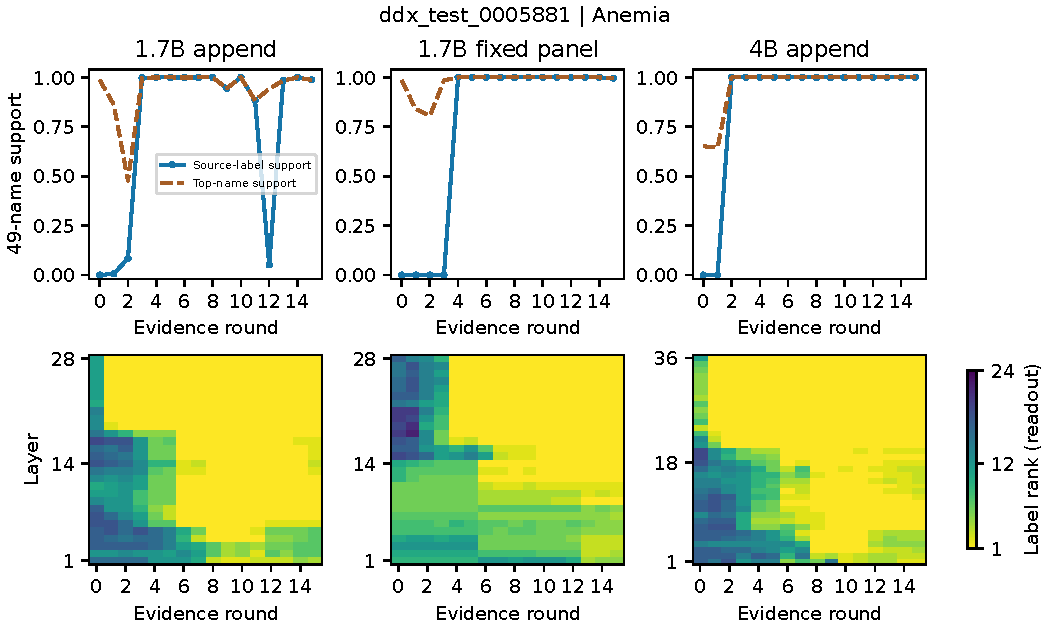
\includegraphics[width=.96\linewidth]{figures/ddx_test_0005881.pdf}\end{center}

{\small\begin{longtable}{>{\raggedright\arraybackslash}p{.07\textwidth}>{\raggedright\arraybackslash}p{.415\textwidth}>{\raggedright\arraybackslash}p{.415\textwidth}}\toprule Round & Newly revealed source evidence & Native top / label support / final-layer probe top \\ \midrule\endhead

0 & Are you experiencing shortness of breath or difficulty breathing in a significant way? Yes & 1.7B append: Acute COPD exacerbation / infection / 0.0000 / Bronchitis\newline 1.7B panel: Acute pulmonary edema / 0.0000 / Guillain-Barr\'{e} syndrome\newline 4B append: Acute rhinosinusitis / 0.0000 / Bronchitis \\ 

1 & Have you recently had stools that were black (like coal)? Yes & 1.7B append: Acute COPD exacerbation / infection / 0.0065 / Anemia\newline 1.7B panel: Acute pulmonary edema / 0.0000 / Guillain-Barr\'{e} syndrome\newline 4B append: Pulmonary embolism / 0.0006 / Anemia \\ 

2 & Is your BMI less than 18.5, or are you underweight? Yes & 1.7B append: Acute COPD exacerbation / infection / 0.0840 / Anemia\newline 1.7B panel: Acute pulmonary edema / 0.0000 / Guillain-Barr\'{e} syndrome\newline 4B append: Anemia / 0.9999 / Anemia \\ 

3 & Do you have any family members who have been diagnosed with anemia? Yes & 1.7B append: Anemia / 0.9983 / Anemia\newline 1.7B panel: Acute pulmonary edema / 0.0000 / Guillain-Barr\'{e} syndrome\newline 4B append: Anemia / 1.0000 / Anemia \\ 

4 & Have you ever had a diagnosis of anemia? Yes & 1.7B append: Anemia / 0.9998 / Anemia\newline 1.7B panel: Anemia / 1.0000 / Anemia\newline 4B append: Anemia / 1.0000 / Anemia \\ 

5 & Do you feel so tired that you are unable to do your usual activities or are you stuck in your bed all day long? Yes & 1.7B append: Anemia / 1.0000 / Anemia\newline 1.7B panel: Anemia / 1.0000 / Anemia\newline 4B append: Anemia / 1.0000 / Anemia \\ 

6 & Do you have pain somewhere, related to your reason for consulting? Yes; Characterize your pain: sensitive; tugging; exhausting; Do you feel pain somewhere? back of head; top of the head; forehead; How intense is the pain? Recorded scale value 3 on the dataset's 0-10 scale; endpoint meanings are unspecified; Does the pain radiate to another location? nowhere; How precisely is the pain located? Recorded scale value 5 on the dataset's 0-10 scale; endpoint meanings are unspecified; How fast did the pain appear? Recorded scale value 4 on the dataset's 0-10 scale; endpoint meanings are unspecified & 1.7B append: Anemia / 0.9992 / Anemia\newline 1.7B panel: Anemia / 1.0000 / Anemia\newline 4B append: Anemia / 1.0000 / Anemia \\ 

7 & Do you have chronic kidney failure? Yes & 1.7B append: Anemia / 0.9999 / Anemia\newline 1.7B panel: Anemia / 1.0000 / Anemia\newline 4B append: Anemia / 1.0000 / Anemia \\ 

8 & Do you think you are pregnant or are you currently pregnant? Yes & 1.7B append: Anemia / 1.0000 / Anemia\newline 1.7B panel: Anemia / 1.0000 / Anemia\newline 4B append: Anemia / 1.0000 / Anemia \\ 

9 & Do you feel slightly dizzy or lightheaded? Yes & 1.7B append: Anemia / 0.9450 / Anemia\newline 1.7B panel: Anemia / 1.0000 / Anemia\newline 4B append: Anemia / 1.0000 / Anemia \\ 

10 & Are you taking any new oral anticoagulants ((NOACs)? Yes & 1.7B append: Anemia / 1.0000 / Anemia\newline 1.7B panel: Anemia / 1.0000 / Anemia\newline 4B append: Anemia / 1.0000 / Anemia \\ 

11 & Do you have very abundant or very long menstruation periods? Yes & 1.7B append: Anemia / 0.8839 / Anemia\newline 1.7B panel: Anemia / 1.0000 / Anemia\newline 4B append: Anemia / 1.0000 / Anemia \\ 

12 & Do you feel lightheaded and dizzy or do you feel like you are about to faint? Yes & 1.7B append: Acute pulmonary edema / 0.0515 / Anemia\newline 1.7B panel: Anemia / 1.0000 / Anemia\newline 4B append: Anemia / 1.0000 / Anemia \\ 

13 & Have you traveled out of the country in the last 4 weeks? Central America & 1.7B append: Anemia / 0.9843 / Anemia\newline 1.7B panel: Anemia / 1.0000 / Anemia\newline 4B append: Anemia / 1.0000 / Anemia \\ 

14 & Do you constantly feel fatigued or do you have non-restful sleep? Yes & 1.7B append: Anemia / 0.9996 / Anemia\newline 1.7B panel: Anemia / 1.0000 / Anemia\newline 4B append: Anemia / 1.0000 / Anemia \\ 

15 & Do you have a poor diet? Yes & 1.7B append: Anemia / 0.9875 / Anemia\newline 1.7B panel: Anemia / 0.9959 / Anemia\newline 4B append: Anemia / 1.0000 / Anemia \\ 

\bottomrule\end{longtable}}

\clearpage\subsection{ddx\_test\_0006854 -- Anemia}
\label{case:ddx_test_0006854}

Source label: Anemia. Family: systemic. Evidence updates: 9. All facts below are source-recorded; their order is acquisition order.

\begin{center}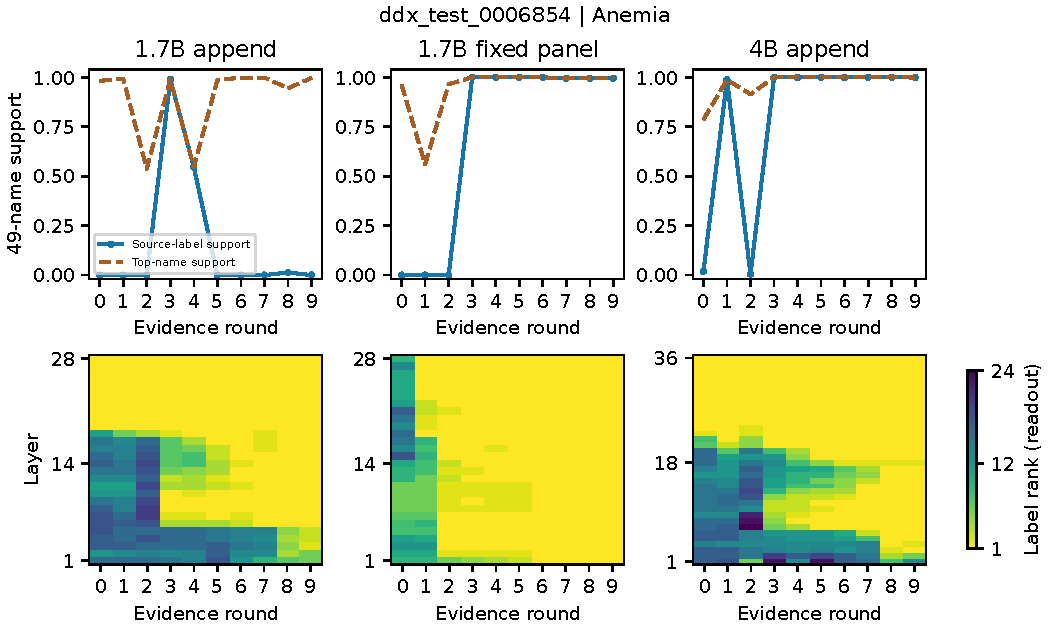
\includegraphics[width=.96\linewidth]{figures/ddx_test_0006854.pdf}\end{center}

{\small\begin{longtable}{>{\raggedright\arraybackslash}p{.07\textwidth}>{\raggedright\arraybackslash}p{.415\textwidth}>{\raggedright\arraybackslash}p{.415\textwidth}}\toprule Round & Newly revealed source evidence & Native top / label support / final-layer probe top \\ \midrule\endhead

0 & Have you noticed light red blood or blood clots in your stool? Yes & 1.7B append: Pulmonary embolism / 0.0000 / Anemia\newline 1.7B panel: Acute COPD exacerbation / infection / 0.0000 / HIV (initial infection)\newline 4B append: Pulmonary embolism / 0.0191 / Anemia \\ 

1 & Do you have chronic kidney failure? Yes & 1.7B append: Pulmonary embolism / 0.0000 / Anemia\newline 1.7B panel: Acute pulmonary edema / 0.0000 / Anemia\newline 4B append: Anemia / 0.9881 / Anemia \\ 

2 & Do you have pain somewhere, related to your reason for consulting? Yes; Characterize your pain: sensitive; a cramp; Do you feel pain somewhere? back of head; temple(R); How intense is the pain? Recorded scale value 5 on the dataset's 0-10 scale; endpoint meanings are unspecified; Does the pain radiate to another location? nowhere; How precisely is the pain located? Recorded scale value 8 on the dataset's 0-10 scale; endpoint meanings are unspecified; How fast did the pain appear? Recorded scale value 4 on the dataset's 0-10 scale; endpoint meanings are unspecified & 1.7B append: Pulmonary embolism / 0.0000 / Anemia\newline 1.7B panel: Acute COPD exacerbation / infection / 0.0000 / Anemia\newline 4B append: Pulmonary embolism / 0.0041 / Anemia \\ 

3 & Have you ever had a diagnosis of anemia? Yes & 1.7B append: Anemia / 0.9896 / Anemia\newline 1.7B panel: Anemia / 1.0000 / Anemia\newline 4B append: Anemia / 1.0000 / Anemia \\ 

4 & Is your BMI less than 18.5, or are you underweight? Yes & 1.7B append: Anemia / 0.5457 / Anemia\newline 1.7B panel: Anemia / 1.0000 / Anemia\newline 4B append: Anemia / 1.0000 / Anemia \\ 

5 & Have you recently had stools that were black (like coal)? Yes & 1.7B append: Pulmonary embolism / 0.0000 / Anemia\newline 1.7B panel: Anemia / 1.0000 / Anemia\newline 4B append: Anemia / 1.0000 / Anemia \\ 

6 & Have you traveled out of the country in the last 4 weeks? South Africa & 1.7B append: Pulmonary embolism / 0.0000 / Anemia\newline 1.7B panel: Anemia / 1.0000 / Anemia\newline 4B append: Anemia / 1.0000 / Anemia \\ 

7 & Do you have a poor diet? Yes & 1.7B append: Pulmonary embolism / 0.0000 / Anemia\newline 1.7B panel: Anemia / 0.9957 / Anemia\newline 4B append: Anemia / 1.0000 / Anemia \\ 

8 & Do you have any family members who have been diagnosed with anemia? Yes & 1.7B append: Pulmonary embolism / 0.0129 / Anemia\newline 1.7B panel: Anemia / 0.9957 / Anemia\newline 4B append: Anemia / 1.0000 / Anemia \\ 

9 & Are you taking any new oral anticoagulants ((NOACs)? Yes & 1.7B append: Pulmonary embolism / 0.0000 / Anemia\newline 1.7B panel: Anemia / 0.9957 / Anemia\newline 4B append: Anemia / 0.9997 / Anemia \\ 

\bottomrule\end{longtable}}

\clearpage\subsection{ddx\_test\_0017896 -- HIV (initial infection)}
\label{case:ddx_test_0017896}

Source label: HIV (initial infection). Family: systemic. Evidence updates: 11. All facts below are source-recorded; their order is acquisition order.

\begin{center}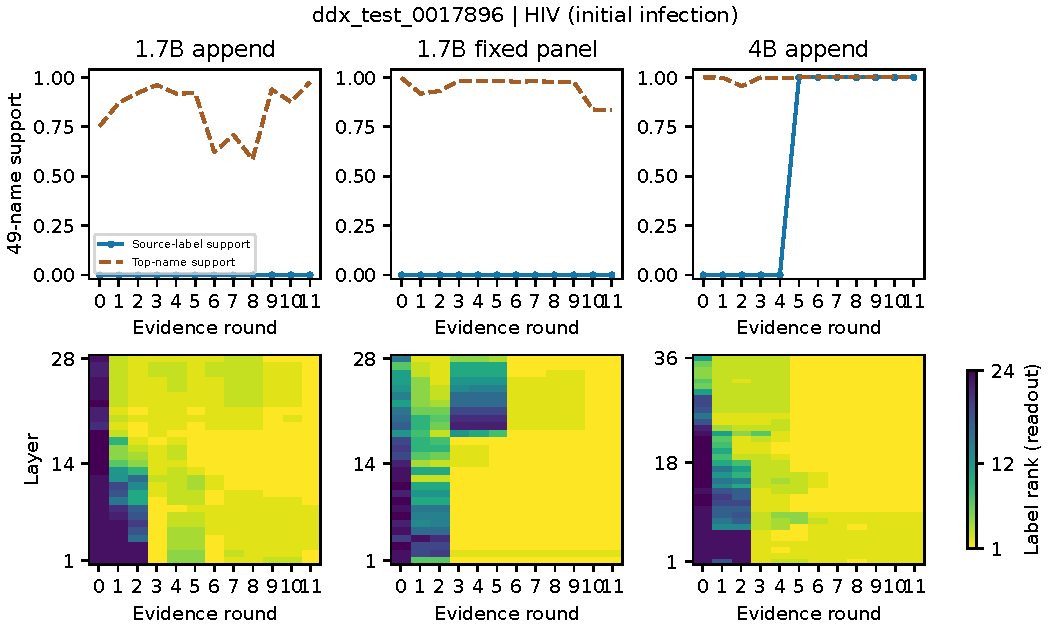
\includegraphics[width=.96\linewidth]{figures/ddx_test_0017896.pdf}\end{center}

{\small\begin{longtable}{>{\raggedright\arraybackslash}p{.07\textwidth}>{\raggedright\arraybackslash}p{.415\textwidth}>{\raggedright\arraybackslash}p{.415\textwidth}}\toprule Round & Newly revealed source evidence & Native top / label support / final-layer probe top \\ \midrule\endhead

0 & Do you have a sore throat? Yes & 1.7B append: Acute rhinosinusitis / 0.0000 / URTI\newline 1.7B panel: Acute COPD exacerbation / infection / 0.0000 / URTI\newline 4B append: Viral pharyngitis / 0.0000 / Viral pharyngitis \\ 

1 & Do you have any lesions, redness or problems on your skin that you believe are related to the condition you are consulting for? Yes; What color is the rash? pale; Do your lesions peel off? No; Is the rash swollen? Recorded scale value 2 on the dataset's 0-10 scale; endpoint meanings are unspecified; Where is the affected region located? lower gum; upper gum; internal cheek(R); internal cheek(L); bottom lip(R); How intense is the pain caused by the rash? Recorded scale value 5 on the dataset's 0-10 scale; endpoint meanings are unspecified; Is the lesion (or are the lesions) larger than 1cm? Yes; How severe is the itching? Recorded scale value 0 on the dataset's 0-10 scale; endpoint meanings are unspecified & 1.7B append: Viral pharyngitis / 0.0000 / URTI\newline 1.7B panel: Acute COPD exacerbation / infection / 0.0000 / URTI\newline 4B append: Viral pharyngitis / 0.0000 / Viral pharyngitis \\ 

2 & Have you had an involuntary weight loss over the last 3 months? Yes & 1.7B append: Acute rhinosinusitis / 0.0000 / URTI\newline 1.7B panel: Acute COPD exacerbation / infection / 0.0000 / URTI\newline 4B append: Viral pharyngitis / 0.0000 / SLE \\ 

3 & Do you have pain somewhere, related to your reason for consulting? Yes; Characterize your pain: tedious; sensitive; exhausting; Do you feel pain somewhere? back of head; top of the head; forehead; occiput; temple(L); How intense is the pain? Recorded scale value 6 on the dataset's 0-10 scale; endpoint meanings are unspecified; Does the pain radiate to another location? nowhere; How precisely is the pain located? Recorded scale value 8 on the dataset's 0-10 scale; endpoint meanings are unspecified; How fast did the pain appear? Recorded scale value 4 on the dataset's 0-10 scale; endpoint meanings are unspecified & 1.7B append: Acute rhinosinusitis / 0.0000 / URTI\newline 1.7B panel: Acute COPD exacerbation / infection / 0.0000 / SLE\newline 4B append: Viral pharyngitis / 0.0000 / Viral pharyngitis \\ 

4 & Have you had unprotected sex with more than one partner in the last 6 months? Yes & 1.7B append: Acute rhinosinusitis / 0.0000 / URTI\newline 1.7B panel: Acute COPD exacerbation / infection / 0.0000 / SLE\newline 4B append: Viral pharyngitis / 0.0000 / Viral pharyngitis \\ 

5 & Have you had sexual intercourse with an HIV-positive partner in the past 12 months? Yes & 1.7B append: Acute rhinosinusitis / 0.0000 / URTI\newline 1.7B panel: Acute COPD exacerbation / infection / 0.0000 / SLE\newline 4B append: HIV (initial infection) / 1.0000 / HIV (initial infection) \\ 

6 & Have you had significantly increased sweating? Yes & 1.7B append: Acute rhinosinusitis / 0.0000 / URTI\newline 1.7B panel: Acute COPD exacerbation / infection / 0.0000 / HIV (initial infection)\newline 4B append: HIV (initial infection) / 1.0000 / HIV (initial infection) \\ 

7 & Do you have diffuse (widespread) muscle pain? Yes & 1.7B append: Acute rhinosinusitis / 0.0000 / URTI\newline 1.7B panel: Acute COPD exacerbation / infection / 0.0000 / HIV (initial infection)\newline 4B append: HIV (initial infection) / 1.0000 / HIV (initial infection) \\ 

8 & Are you currently using intravenous drugs? Yes & 1.7B append: Acute rhinosinusitis / 0.0000 / URTI\newline 1.7B panel: Acute COPD exacerbation / infection / 0.0000 / HIV (initial infection)\newline 4B append: HIV (initial infection) / 1.0000 / HIV (initial infection) \\ 

9 & Have you traveled out of the country in the last 4 weeks? No & 1.7B append: Acute rhinosinusitis / 0.0000 / HIV (initial infection)\newline 1.7B panel: Acute COPD exacerbation / infection / 0.0000 / HIV (initial infection)\newline 4B append: HIV (initial infection) / 1.0000 / HIV (initial infection) \\ 

10 & Do you have swollen or painful lymph nodes? Yes & 1.7B append: Acute rhinosinusitis / 0.0000 / HIV (initial infection)\newline 1.7B panel: Acute COPD exacerbation / infection / 0.0000 / HIV (initial infection)\newline 4B append: HIV (initial infection) / 1.0000 / HIV (initial infection) \\ 

11 & Do you have a fever (either felt or measured with a thermometer)? Yes & 1.7B append: Acute rhinosinusitis / 0.0000 / HIV (initial infection)\newline 1.7B panel: Acute COPD exacerbation / infection / 0.0000 / HIV (initial infection)\newline 4B append: HIV (initial infection) / 1.0000 / HIV (initial infection) \\ 

\bottomrule\end{longtable}}

\clearpage\subsection{ddx\_test\_0027885 -- Pancreatic neoplasm}
\label{case:ddx_test_0027885}

Source label: Pancreatic neoplasm. Family: digestive. Evidence updates: 9. All facts below are source-recorded; their order is acquisition order.

\begin{center}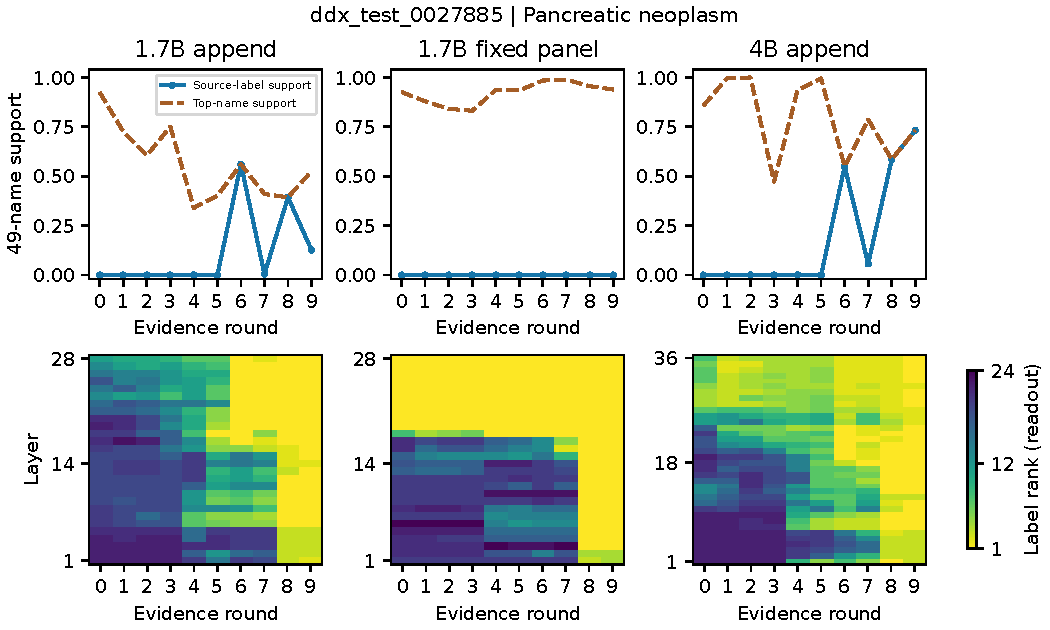
\includegraphics[width=.96\linewidth]{figures/ddx_test_0027885.pdf}\end{center}

{\small\begin{longtable}{>{\raggedright\arraybackslash}p{.07\textwidth}>{\raggedright\arraybackslash}p{.415\textwidth}>{\raggedright\arraybackslash}p{.415\textwidth}}\toprule Round & Newly revealed source evidence & Native top / label support / final-layer probe top \\ \midrule\endhead

0 & Have you had diarrhea or an increase in stool frequency? Yes & 1.7B append: Acute COPD exacerbation / infection / 0.0000 / Bronchitis\newline 1.7B panel: Acute COPD exacerbation / infection / 0.0000 / Pancreatic neoplasm\newline 4B append: Acute rhinosinusitis / 0.0000 / URTI \\ 

1 & Do you have diabetes? Yes & 1.7B append: Acute COPD exacerbation / infection / 0.0000 / Bronchitis\newline 1.7B panel: Acute COPD exacerbation / infection / 0.0000 / Pancreatic neoplasm\newline 4B append: Influenza / 0.0000 / URTI \\ 

2 & Have you traveled out of the country in the last 4 weeks? No & 1.7B append: Acute COPD exacerbation / infection / 0.0000 / HIV (initial infection)\newline 1.7B panel: Acute COPD exacerbation / infection / 0.0000 / Pancreatic neoplasm\newline 4B append: Influenza / 0.0000 / URTI \\ 

3 & Are you significantly overweight compared to people of the same height as you? Yes & 1.7B append: Acute COPD exacerbation / infection / 0.0000 / Anemia\newline 1.7B panel: Acute COPD exacerbation / infection / 0.0000 / Pancreatic neoplasm\newline 4B append: Influenza / 0.0000 / URTI \\ 

4 & Do you have pain somewhere, related to your reason for consulting? Yes; Characterize your pain: a cramp; Do you feel pain somewhere? flank(L); epigastric; How intense is the pain? Recorded scale value 1 on the dataset's 0-10 scale; endpoint meanings are unspecified; Does the pain radiate to another location? nowhere; How precisely is the pain located? Recorded scale value 1 on the dataset's 0-10 scale; endpoint meanings are unspecified; How fast did the pain appear? Recorded scale value 5 on the dataset's 0-10 scale; endpoint meanings are unspecified & 1.7B append: Acute rhinosinusitis / 0.0006 / Inguinal hernia\newline 1.7B panel: Acute COPD exacerbation / infection / 0.0000 / Pancreatic neoplasm\newline 4B append: Bronchitis / 0.0008 / Boerhaave \\ 

5 & Do you smoke cigarettes? Yes & 1.7B append: Acute rhinosinusitis / 0.0001 / Inguinal hernia\newline 1.7B panel: Acute COPD exacerbation / infection / 0.0000 / Pancreatic neoplasm\newline 4B append: Bronchitis / 0.0000 / Boerhaave \\ 

6 & Do you have chronic pancreatitis? Yes & 1.7B append: Pancreatic neoplasm / 0.5602 / Pancreatic neoplasm\newline 1.7B panel: Acute COPD exacerbation / infection / 0.0000 / Pancreatic neoplasm\newline 4B append: Pancreatic neoplasm / 0.5491 / Boerhaave \\ 

7 & Do you have a cough? Yes & 1.7B append: Acute rhinosinusitis / 0.0052 / Inguinal hernia\newline 1.7B panel: Acute COPD exacerbation / infection / 0.0000 / Pancreatic neoplasm\newline 4B append: Bronchitis / 0.0570 / Boerhaave \\ 

8 & Do you have any lesions, redness or problems on your skin that you believe are related to the condition you are consulting for? Yes; What color is the rash? yellow; Do your lesions peel off? No; Is the rash swollen? Recorded scale value 0 on the dataset's 0-10 scale; endpoint meanings are unspecified; Where is the affected region located? epigastric; How intense is the pain caused by the rash? Recorded scale value 2 on the dataset's 0-10 scale; endpoint meanings are unspecified; Is the lesion (or are the lesions) larger than 1cm? Yes; How severe is the itching? Recorded scale value 3 on the dataset's 0-10 scale; endpoint meanings are unspecified & 1.7B append: Pancreatic neoplasm / 0.3933 / Pancreatic neoplasm\newline 1.7B panel: Acute COPD exacerbation / infection / 0.0000 / Pancreatic neoplasm\newline 4B append: Pancreatic neoplasm / 0.5849 / Boerhaave \\ 

9 & Have you had an involuntary weight loss over the last 3 months? Yes & 1.7B append: Bronchiolitis / 0.1266 / Pancreatic neoplasm\newline 1.7B panel: Acute COPD exacerbation / infection / 0.0000 / Pancreatic neoplasm\newline 4B append: Pancreatic neoplasm / 0.7317 / Pancreatic neoplasm \\ 

\bottomrule\end{longtable}}

\clearpage\subsection{ddx\_test\_0032489 -- Acute dystonic reactions}
\label{case:ddx_test_0032489}

Source label: Acute dystonic reactions. Family: neurologic. Evidence updates: 7. All facts below are source-recorded; their order is acquisition order.

\begin{center}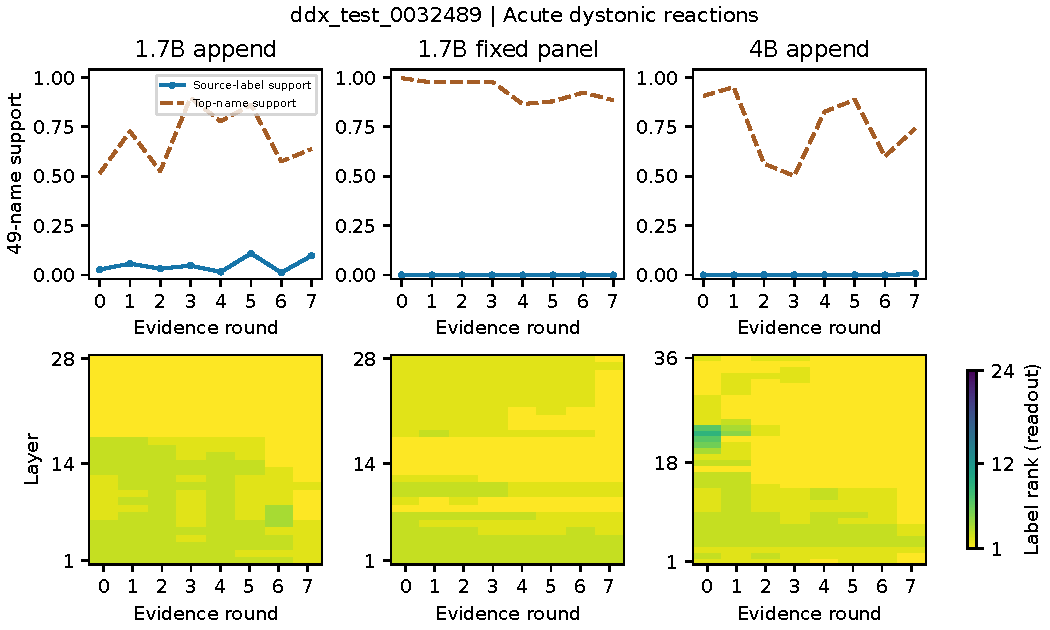
\includegraphics[width=.96\linewidth]{figures/ddx_test_0032489.pdf}\end{center}

{\small\begin{longtable}{>{\raggedright\arraybackslash}p{.07\textwidth}>{\raggedright\arraybackslash}p{.415\textwidth}>{\raggedright\arraybackslash}p{.415\textwidth}}\toprule Round & Newly revealed source evidence & Native top / label support / final-layer probe top \\ \midrule\endhead

0 & Do you feel that muscle spasms or soreness in your neck are keeping you from turning your head to one side? Yes & 1.7B append: Acute laryngitis / 0.0277 / Acute dystonic reactions\newline 1.7B panel: Acute COPD exacerbation / infection / 0.0001 / Myasthenia gravis\newline 4B append: Acute otitis media / 0.0000 / URTI \\ 

1 & Do you have a hard time opening/raising one or both eyelids? Yes & 1.7B append: Acute laryngitis / 0.0579 / Acute dystonic reactions\newline 1.7B panel: Acute COPD exacerbation / infection / 0.0000 / Myasthenia gravis\newline 4B append: Acute otitis media / 0.0000 / Acute dystonic reactions \\ 

2 & Do you regularly take stimulant drugs? Yes & 1.7B append: Acute laryngitis / 0.0326 / Acute dystonic reactions\newline 1.7B panel: Acute COPD exacerbation / infection / 0.0001 / Myasthenia gravis\newline 4B append: Acute laryngitis / 0.0013 / Myasthenia gravis \\ 

3 & Do you suddenly have difficulty or an inability to open your mouth or have jaw pain when opening it? Yes & 1.7B append: Acute laryngitis / 0.0475 / Acute dystonic reactions\newline 1.7B panel: Acute COPD exacerbation / infection / 0.0001 / Myasthenia gravis\newline 4B append: Acute laryngitis / 0.0009 / Myasthenia gravis \\ 

4 & Have you ever felt like you were suffocating for a very short time associated with inability to breathe or speak? Yes & 1.7B append: Acute laryngitis / 0.0159 / Acute dystonic reactions\newline 1.7B panel: Acute COPD exacerbation / infection / 0.0001 / Myasthenia gravis\newline 4B append: Panic attack / 0.0000 / Acute dystonic reactions \\ 

5 & Do you have trouble keeping your tongue in your mouth? Yes & 1.7B append: Acute laryngitis / 0.1095 / Acute dystonic reactions\newline 1.7B panel: Acute COPD exacerbation / infection / 0.0001 / Myasthenia gravis\newline 4B append: Panic attack / 0.0004 / Acute dystonic reactions \\ 

6 & Have you traveled out of the country in the last 4 weeks? No & 1.7B append: Acute laryngitis / 0.0127 / Acute dystonic reactions\newline 1.7B panel: Acute COPD exacerbation / infection / 0.0001 / Myasthenia gravis\newline 4B append: Panic attack / 0.0000 / Acute dystonic reactions \\ 

7 & Have you been treated in hospital recently for nausea, agitation, intoxication or aggressive behavior and received medication via an intravenous or intramuscular route? Yes & 1.7B append: Acute laryngitis / 0.0977 / Acute dystonic reactions\newline 1.7B panel: Acute COPD exacerbation / infection / 0.0000 / Acute dystonic reactions\newline 4B append: Panic attack / 0.0068 / Acute dystonic reactions \\ 

\bottomrule\end{longtable}}

\clearpage\subsection{ddx\_test\_0037913 -- Pericarditis}
\label{case:ddx_test_0037913}

Source label: Pericarditis. Family: cardiovascular. Evidence updates: 4. All facts below are source-recorded; their order is acquisition order.

\begin{center}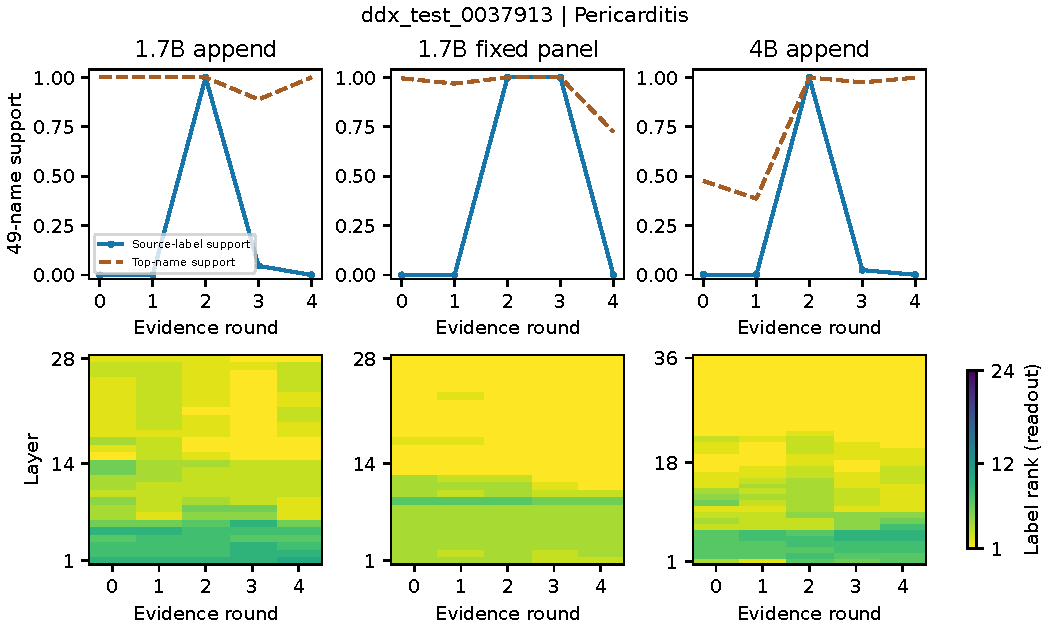
\includegraphics[width=.96\linewidth]{figures/ddx_test_0037913.pdf}\end{center}

{\small\begin{longtable}{>{\raggedright\arraybackslash}p{.07\textwidth}>{\raggedright\arraybackslash}p{.415\textwidth}>{\raggedright\arraybackslash}p{.415\textwidth}}\toprule Round & Newly revealed source evidence & Native top / label support / final-layer probe top \\ \midrule\endhead

0 & Do you have pain somewhere, related to your reason for consulting? Yes; Characterize your pain: a knife stroke; sharp; Do you feel pain somewhere? lower chest; breast(R); How intense is the pain? Recorded scale value 6 on the dataset's 0-10 scale; endpoint meanings are unspecified; Does the pain radiate to another location? thoracic spine; posterior chest wall(R); How precisely is the pain located? Recorded scale value 8 on the dataset's 0-10 scale; endpoint meanings are unspecified; How fast did the pain appear? Recorded scale value 6 on the dataset's 0-10 scale; endpoint meanings are unspecified & 1.7B append: Boerhaave / 0.0000 / Pulmonary embolism\newline 1.7B panel: Acute COPD exacerbation / infection / 0.0000 / Pericarditis\newline 4B append: Bronchospasm / acute asthma exacerbation / 0.0020 / Pericarditis \\ 

1 & Do you have pain that is increased when you breathe in deeply? Yes & 1.7B append: Boerhaave / 0.0000 / Pulmonary embolism\newline 1.7B panel: Acute COPD exacerbation / infection / 0.0000 / Pericarditis\newline 4B append: Pneumonia / 0.0025 / Pericarditis \\ 

2 & Have you ever had a pericarditis? Yes & 1.7B append: Pericarditis / 1.0000 / SLE\newline 1.7B panel: Pericarditis / 1.0000 / Pericarditis\newline 4B append: Pericarditis / 0.9994 / Pericarditis \\ 

3 & Have you recently had a viral infection? Yes & 1.7B append: Acute laryngitis / 0.0467 / Pericarditis\newline 1.7B panel: Pericarditis / 1.0000 / Pericarditis\newline 4B append: Myocarditis / 0.0252 / Pericarditis \\ 

4 & Have you traveled out of the country in the last 4 weeks? No & 1.7B append: Boerhaave / 0.0000 / Pericarditis\newline 1.7B panel: Acute COPD exacerbation / infection / 0.0013 / Pericarditis\newline 4B append: Myocarditis / 0.0014 / Pericarditis \\ 

\bottomrule\end{longtable}}

\clearpage\subsection{ddx\_test\_0041136 -- Acute otitis media}
\label{case:ddx_test_0041136}

Source label: Acute otitis media. Family: ent. Evidence updates: 5. All facts below are source-recorded; their order is acquisition order.

\begin{center}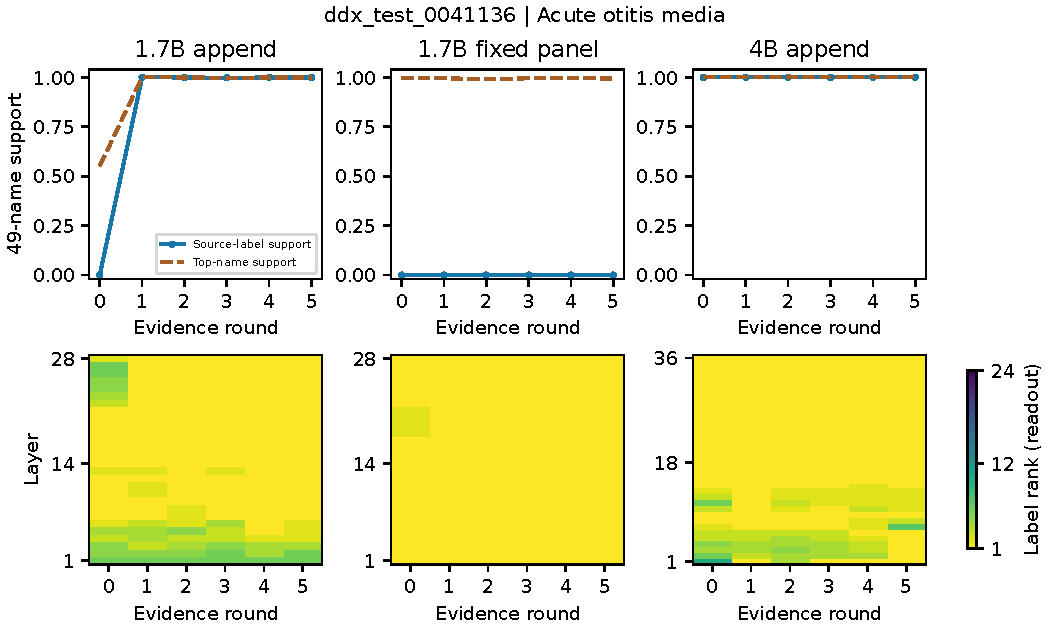
\includegraphics[width=.96\linewidth]{figures/ddx_test_0041136.pdf}\end{center}

{\small\begin{longtable}{>{\raggedright\arraybackslash}p{.07\textwidth}>{\raggedright\arraybackslash}p{.415\textwidth}>{\raggedright\arraybackslash}p{.415\textwidth}}\toprule Round & Newly revealed source evidence & Native top / label support / final-layer probe top \\ \midrule\endhead

0 & Do you have pain somewhere, related to your reason for consulting? Yes; Characterize your pain: sensitive; sharp; Do you feel pain somewhere? ear(R); How intense is the pain? Recorded scale value 6 on the dataset's 0-10 scale; endpoint meanings are unspecified; Does the pain radiate to another location? nowhere; How precisely is the pain located? Recorded scale value 9 on the dataset's 0-10 scale; endpoint meanings are unspecified; How fast did the pain appear? Recorded scale value 3 on the dataset's 0-10 scale; endpoint meanings are unspecified & 1.7B append: Acute laryngitis / 0.0000 / Cluster headache\newline 1.7B panel: Acute COPD exacerbation / infection / 0.0000 / Acute otitis media\newline 4B append: Acute otitis media / 1.0000 / Acute otitis media \\ 

1 & Are you currently being treated or have you recently been treated with an oral antibiotic for an ear infection? Yes & 1.7B append: Acute otitis media / 1.0000 / Acute otitis media\newline 1.7B panel: Acute COPD exacerbation / infection / 0.0001 / Acute otitis media\newline 4B append: Acute otitis media / 1.0000 / Acute otitis media \\ 

2 & Do you have a fever (either felt or measured with a thermometer)? Yes & 1.7B append: Acute otitis media / 0.9998 / Acute otitis media\newline 1.7B panel: Acute COPD exacerbation / infection / 0.0001 / Acute otitis media\newline 4B append: Acute otitis media / 1.0000 / Acute otitis media \\ 

3 & Do you have a cough? Yes & 1.7B append: Acute otitis media / 0.9986 / Acute otitis media\newline 1.7B panel: Acute COPD exacerbation / infection / 0.0000 / Acute otitis media\newline 4B append: Acute otitis media / 1.0000 / Acute otitis media \\ 

4 & Are your vaccinations up to date? Yes & 1.7B append: Acute otitis media / 0.9995 / Acute otitis media\newline 1.7B panel: Acute COPD exacerbation / infection / 0.0000 / Acute otitis media\newline 4B append: Acute otitis media / 1.0000 / Acute otitis media \\ 

5 & Have you traveled out of the country in the last 4 weeks? No & 1.7B append: Acute otitis media / 0.9996 / Acute otitis media\newline 1.7B panel: Acute COPD exacerbation / infection / 0.0000 / Acute otitis media\newline 4B append: Acute otitis media / 1.0000 / Acute otitis media \\ 

\bottomrule\end{longtable}}

\clearpage\subsection{ddx\_test\_0042118 -- Bronchitis}
\label{case:ddx_test_0042118}

Source label: Bronchitis. Family: respiratory. Evidence updates: 8. All facts below are source-recorded; their order is acquisition order.

\begin{center}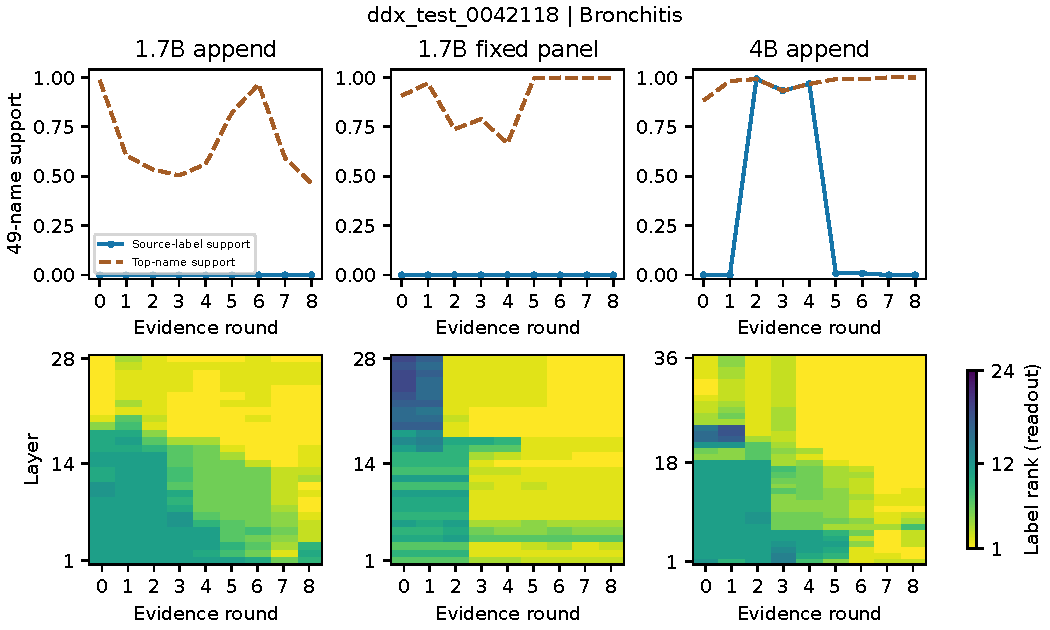
\includegraphics[width=.96\linewidth]{figures/ddx_test_0042118.pdf}\end{center}

{\small\begin{longtable}{>{\raggedright\arraybackslash}p{.07\textwidth}>{\raggedright\arraybackslash}p{.415\textwidth}>{\raggedright\arraybackslash}p{.415\textwidth}}\toprule Round & Newly revealed source evidence & Native top / label support / final-layer probe top \\ \midrule\endhead

0 & Are your symptoms more prominent at night? Yes & 1.7B append: Acute COPD exacerbation / infection / 0.0000 / Bronchitis\newline 1.7B panel: Acute COPD exacerbation / infection / 0.0000 / Guillain-Barr\'{e} syndrome\newline 4B append: Acute rhinosinusitis / 0.0006 / URTI \\ 

1 & Have you traveled out of the country in the last 4 weeks? No & 1.7B append: Acute rhinosinusitis / 0.0000 / Acute otitis media\newline 1.7B panel: Acute COPD exacerbation / infection / 0.0000 / Guillain-Barr\'{e} syndrome\newline 4B append: Acute rhinosinusitis / 0.0001 / URTI \\ 

2 & Have you noticed a wheezing sound when you exhale? Yes & 1.7B append: Bronchiolitis / 0.0000 / Bronchospasm / acute asthma exacerbation\newline 1.7B panel: Whooping cough / 0.0000 / Bronchospasm / acute asthma exacerbation\newline 4B append: Bronchitis / 0.9918 / Bronchospasm / acute asthma exacerbation \\ 

3 & Do you have pain somewhere, related to your reason for consulting? Yes; Characterize your pain: sensitive; Do you feel pain somewhere? lower chest; side of the chest(R); upper chest; breast(L); posterior chest wall(R); How intense is the pain? Recorded scale value 5 on the dataset's 0-10 scale; endpoint meanings are unspecified; Does the pain radiate to another location? nowhere; How precisely is the pain located? Recorded scale value 4 on the dataset's 0-10 scale; endpoint meanings are unspecified; How fast did the pain appear? Recorded scale value 1 on the dataset's 0-10 scale; endpoint meanings are unspecified & 1.7B append: Bronchospasm / acute asthma exacerbation / 0.0000 / Bronchitis\newline 1.7B panel: Acute COPD exacerbation / infection / 0.0000 / Bronchospasm / acute asthma exacerbation\newline 4B append: Bronchitis / 0.9327 / Bronchospasm / acute asthma exacerbation \\ 

4 & Do you have a cough that produces colored or more abundant sputum than usual? Yes & 1.7B append: Bronchospasm / acute asthma exacerbation / 0.0000 / Bronchitis\newline 1.7B panel: Acute COPD exacerbation / infection / 0.0000 / Bronchospasm / acute asthma exacerbation\newline 4B append: Bronchitis / 0.9668 / Bronchitis \\ 

5 & Do you have a chronic obstructive pulmonary disease (COPD)? Yes & 1.7B append: Bronchospasm / acute asthma exacerbation / 0.0000 / Bronchitis\newline 1.7B panel: Acute COPD exacerbation / infection / 0.0000 / Bronchospasm / acute asthma exacerbation\newline 4B append: Acute COPD exacerbation / infection / 0.0086 / Bronchitis \\ 

6 & Do you have a cough? Yes & 1.7B append: Bronchospasm / acute asthma exacerbation / 0.0000 / Bronchospasm / acute asthma exacerbation\newline 1.7B panel: Acute COPD exacerbation / infection / 0.0000 / Bronchitis\newline 4B append: Acute COPD exacerbation / infection / 0.0091 / Bronchitis \\ 

7 & Are you experiencing shortness of breath or difficulty breathing in a significant way? Yes & 1.7B append: Acute COPD exacerbation / infection / 0.0000 / Bronchitis\newline 1.7B panel: Acute COPD exacerbation / infection / 0.0000 / Bronchitis\newline 4B append: Acute COPD exacerbation / infection / 0.0000 / Bronchitis \\ 

8 & Are your vaccinations up to date? Yes & 1.7B append: Acute COPD exacerbation / infection / 0.0000 / Bronchitis\newline 1.7B panel: Acute COPD exacerbation / infection / 0.0000 / Bronchitis\newline 4B append: Acute COPD exacerbation / infection / 0.0002 / Bronchitis \\ 

\bottomrule\end{longtable}}

\clearpage\subsection{ddx\_test\_0044249 -- Boerhaave}
\label{case:ddx_test_0044249}

Source label: Boerhaave. Family: digestive. Evidence updates: 5. All facts below are source-recorded; their order is acquisition order.

\begin{center}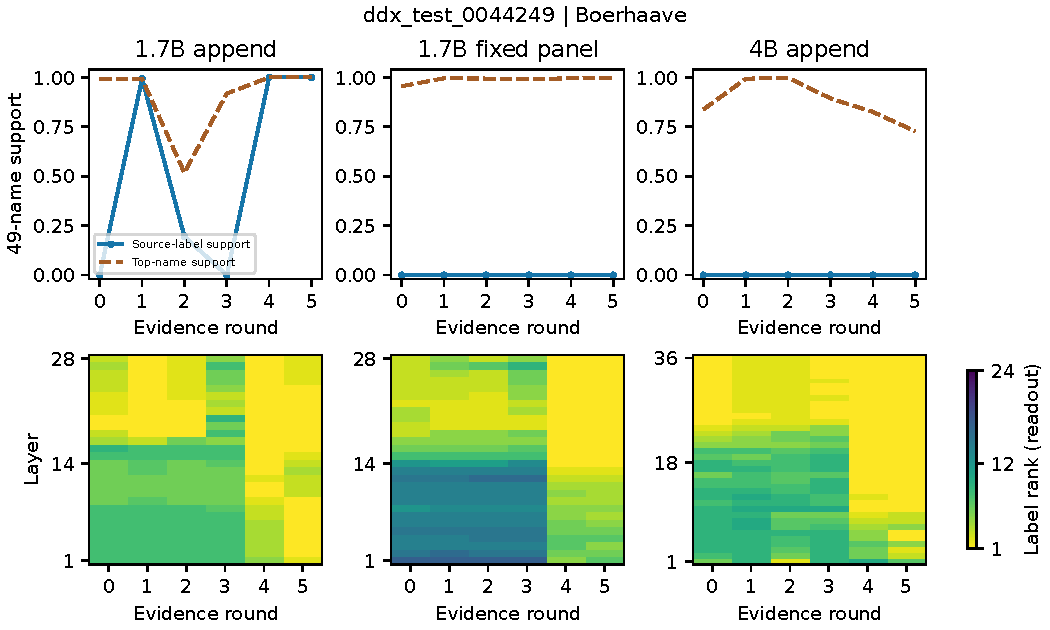
\includegraphics[width=.96\linewidth]{figures/ddx_test_0044249.pdf}\end{center}

{\small\begin{longtable}{>{\raggedright\arraybackslash}p{.07\textwidth}>{\raggedright\arraybackslash}p{.415\textwidth}>{\raggedright\arraybackslash}p{.415\textwidth}}\toprule Round & Newly revealed source evidence & Native top / label support / final-layer probe top \\ \midrule\endhead

0 & Have you vomited several times or have you made several efforts to vomit? Yes & 1.7B append: Acute COPD exacerbation / infection / 0.0000 / GERD\newline 1.7B panel: Acute COPD exacerbation / infection / 0.0000 / Bronchospasm / acute asthma exacerbation\newline 4B append: Acute rhinosinusitis / 0.0000 / Boerhaave \\ 

1 & Are you feeling nauseous or do you feel like vomiting? Yes & 1.7B append: Boerhaave / 0.9932 / Boerhaave\newline 1.7B panel: Acute COPD exacerbation / infection / 0.0000 / Acute dystonic reactions\newline 4B append: Acute rhinosinusitis / 0.0000 / URTI \\ 

2 & Have you traveled out of the country in the last 4 weeks? No & 1.7B append: Acute COPD exacerbation / infection / 0.1947 / GERD\newline 1.7B panel: Acute COPD exacerbation / infection / 0.0000 / Acute dystonic reactions\newline 4B append: Acute rhinosinusitis / 0.0000 / URTI \\ 

3 & Do you drink alcohol excessively or do you have an addiction to alcohol? Yes & 1.7B append: GERD / 0.0000 / GERD\newline 1.7B panel: Acute COPD exacerbation / infection / 0.0000 / Acute dystonic reactions\newline 4B append: Acute rhinosinusitis / 0.0000 / Boerhaave \\ 

4 & Do you have pain somewhere, related to your reason for consulting? Yes; Characterize your pain: heartbreaking; haunting; a knife stroke; violent; sickening; Do you feel pain somewhere? lower chest; flank(R); flank(L); upper chest; epigastric; How intense is the pain? Recorded scale value 6 on the dataset's 0-10 scale; endpoint meanings are unspecified; Does the pain radiate to another location? thoracic spine; scapula(R); scapula(L); How precisely is the pain located? Recorded scale value 2 on the dataset's 0-10 scale; endpoint meanings are unspecified; How fast did the pain appear? Recorded scale value 7 on the dataset's 0-10 scale; endpoint meanings are unspecified & 1.7B append: Boerhaave / 1.0000 / Boerhaave\newline 1.7B panel: Acute COPD exacerbation / infection / 0.0000 / Boerhaave\newline 4B append: Pneumonia / 0.0000 / Boerhaave \\ 

5 & Have you recently thrown up blood or something resembling coffee beans? Yes & 1.7B append: Boerhaave / 0.9999 / GERD\newline 1.7B panel: Acute COPD exacerbation / infection / 0.0000 / Boerhaave\newline 4B append: Pulmonary embolism / 0.0000 / Boerhaave \\ 

\bottomrule\end{longtable}}

\clearpage\subsection{ddx\_test\_0045887 -- URTI}
\label{case:ddx_test_0045887}

Source label: URTI. Family: ent. Evidence updates: 10. All facts below are source-recorded; their order is acquisition order.

\begin{center}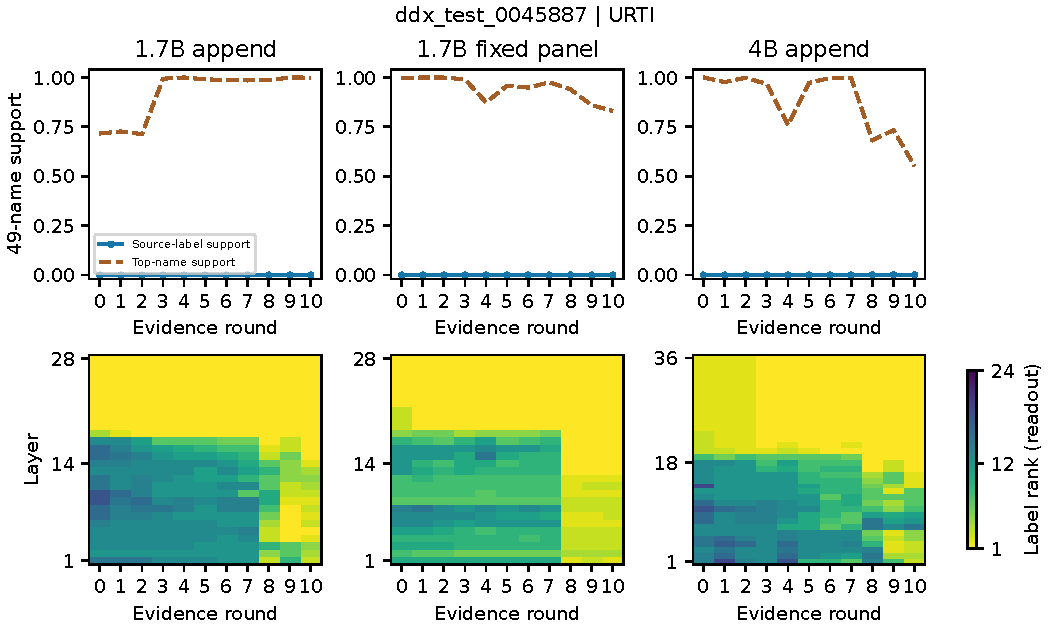
\includegraphics[width=.96\linewidth]{figures/ddx_test_0045887.pdf}\end{center}

{\small\begin{longtable}{>{\raggedright\arraybackslash}p{.07\textwidth}>{\raggedright\arraybackslash}p{.415\textwidth}>{\raggedright\arraybackslash}p{.415\textwidth}}\toprule Round & Newly revealed source evidence & Native top / label support / final-layer probe top \\ \midrule\endhead

0 & Do you have a sore throat? Yes & 1.7B append: Acute rhinosinusitis / 0.0000 / URTI\newline 1.7B panel: Acute COPD exacerbation / infection / 0.0000 / URTI\newline 4B append: Viral pharyngitis / 0.0000 / Viral pharyngitis \\ 

1 & Are you exposed to secondhand cigarette smoke on a daily basis? Yes & 1.7B append: Acute laryngitis / 0.0000 / URTI\newline 1.7B panel: Acute COPD exacerbation / infection / 0.0000 / URTI\newline 4B append: Viral pharyngitis / 0.0000 / Viral pharyngitis \\ 

2 & Do you have diffuse (widespread) muscle pain? Yes & 1.7B append: Acute rhinosinusitis / 0.0000 / URTI\newline 1.7B panel: Acute COPD exacerbation / infection / 0.0000 / URTI\newline 4B append: Viral pharyngitis / 0.0000 / Viral pharyngitis \\ 

3 & Do you have nasal congestion or a clear runny nose? Yes & 1.7B append: Acute rhinosinusitis / 0.0000 / URTI\newline 1.7B panel: Acute COPD exacerbation / infection / 0.0000 / URTI\newline 4B append: Viral pharyngitis / 0.0000 / URTI \\ 

4 & Do you have a cough that produces colored or more abundant sputum than usual? Yes & 1.7B append: Acute rhinosinusitis / 0.0000 / URTI\newline 1.7B panel: Acute COPD exacerbation / infection / 0.0000 / URTI\newline 4B append: Influenza / 0.0002 / URTI \\ 

5 & Have you had significantly increased sweating? Yes & 1.7B append: Acute rhinosinusitis / 0.0000 / URTI\newline 1.7B panel: Acute COPD exacerbation / infection / 0.0000 / URTI\newline 4B append: Influenza / 0.0000 / URTI \\ 

6 & Have you traveled out of the country in the last 4 weeks? No & 1.7B append: Acute rhinosinusitis / 0.0000 / URTI\newline 1.7B panel: Acute COPD exacerbation / infection / 0.0000 / URTI\newline 4B append: Influenza / 0.0000 / URTI \\ 

7 & Do you have a cough? Yes & 1.7B append: Acute rhinosinusitis / 0.0000 / URTI\newline 1.7B panel: Acute COPD exacerbation / infection / 0.0000 / URTI\newline 4B append: Influenza / 0.0000 / URTI \\ 

8 & Do you have pain somewhere, related to your reason for consulting? Yes; Characterize your pain: tedious; Do you feel pain somewhere? forehead; cheek(R); cheek(L); temple(R); How intense is the pain? Recorded scale value 2 on the dataset's 0-10 scale; endpoint meanings are unspecified; Does the pain radiate to another location? nowhere; How precisely is the pain located? Recorded scale value 5 on the dataset's 0-10 scale; endpoint meanings are unspecified; How fast did the pain appear? Recorded scale value 2 on the dataset's 0-10 scale; endpoint meanings are unspecified & 1.7B append: Acute rhinosinusitis / 0.0000 / URTI\newline 1.7B panel: Acute COPD exacerbation / infection / 0.0000 / URTI\newline 4B append: Influenza / 0.0006 / URTI \\ 

9 & Have you been in contact with a person with similar symptoms in the past 2 weeks? Yes & 1.7B append: Acute rhinosinusitis / 0.0000 / URTI\newline 1.7B panel: Acute COPD exacerbation / infection / 0.0000 / URTI\newline 4B append: Viral pharyngitis / 0.0014 / URTI \\ 

10 & Do you live with 4 or more people? Yes & 1.7B append: Acute rhinosinusitis / 0.0000 / URTI\newline 1.7B panel: Acute COPD exacerbation / infection / 0.0000 / URTI\newline 4B append: Viral pharyngitis / 0.0005 / URTI \\ 

\bottomrule\end{longtable}}

\clearpage\subsection{ddx\_test\_0048692 -- Pulmonary embolism}
\label{case:ddx_test_0048692}

Source label: Pulmonary embolism. Family: respiratory. Evidence updates: 6. All facts below are source-recorded; their order is acquisition order.

\begin{center}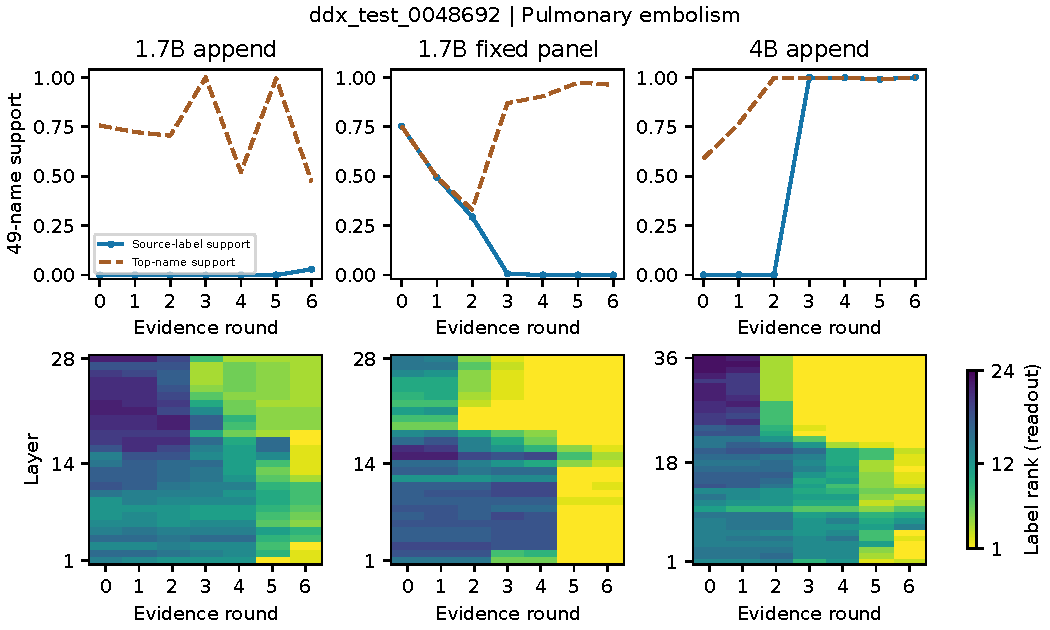
\includegraphics[width=.96\linewidth]{figures/ddx_test_0048692.pdf}\end{center}

{\small\begin{longtable}{>{\raggedright\arraybackslash}p{.07\textwidth}>{\raggedright\arraybackslash}p{.415\textwidth}>{\raggedright\arraybackslash}p{.415\textwidth}}\toprule Round & Newly revealed source evidence & Native top / label support / final-layer probe top \\ \midrule\endhead

0 & Do you have pain that is increased when you breathe in deeply? Yes & 1.7B append: Acute COPD exacerbation / infection / 0.0000 / Bronchitis\newline 1.7B panel: Pulmonary embolism / 0.7534 / SLE\newline 4B append: Acute pulmonary edema / 0.0000 / Bronchitis \\ 

1 & Have you traveled out of the country in the last 4 weeks? No & 1.7B append: Acute rhinosinusitis / 0.0016 / Bronchitis\newline 1.7B panel: Pulmonary embolism / 0.4941 / SLE\newline 4B append: Bronchitis / 0.0025 / Bronchitis \\ 

2 & Have you been coughing up blood? Yes & 1.7B append: Bronchiolitis / 0.0001 / Bronchitis\newline 1.7B panel: Acute COPD exacerbation / infection / 0.2943 / SLE\newline 4B append: Pneumonia / 0.0020 / Pneumonia \\ 

3 & Do you have swelling in one or more areas of your body? Yes; Where is the swelling located? posterior aspect of the ankle(R); posterior aspect of the ankle(L) & 1.7B append: Localized edema / 0.0000 / Acute pulmonary edema\newline 1.7B panel: Acute COPD exacerbation / infection / 0.0067 / SLE\newline 4B append: Pulmonary embolism / 0.9991 / Pulmonary embolism \\ 

4 & Did you lose consciousness? Yes & 1.7B append: Acute pulmonary edema / 0.0009 / Acute pulmonary edema\newline 1.7B panel: Acute COPD exacerbation / infection / 0.0002 / Pulmonary embolism\newline 4B append: Pulmonary embolism / 0.9984 / Pulmonary embolism \\ 

5 & Do you have pain somewhere, related to your reason for consulting? Yes; Characterize your pain: sharp; Do you feel pain somewhere? side of the chest(R); side of the chest(L); scapula(R); scapula(L); posterior chest wall(R); How intense is the pain? Recorded scale value 1 on the dataset's 0-10 scale; endpoint meanings are unspecified; Does the pain radiate to another location? side of the chest(L); upper chest; scapula(R); breast(R); posterior chest wall(L); How precisely is the pain located? Recorded scale value 9 on the dataset's 0-10 scale; endpoint meanings are unspecified; How fast did the pain appear? Recorded scale value 3 on the dataset's 0-10 scale; endpoint meanings are unspecified & 1.7B append: Localized edema / 0.0001 / Acute pulmonary edema\newline 1.7B panel: Acute COPD exacerbation / infection / 0.0000 / Pulmonary embolism\newline 4B append: Pulmonary embolism / 0.9906 / Pulmonary embolism \\ 

6 & Have you ever had deep vein thrombosis (DVT)? Yes & 1.7B append: Acute pulmonary edema / 0.0297 / Spontaneous pneumothorax\newline 1.7B panel: Acute COPD exacerbation / infection / 0.0000 / Pulmonary embolism\newline 4B append: Pulmonary embolism / 1.0000 / Pulmonary embolism \\ 

\bottomrule\end{longtable}}

\clearpage\subsection{ddx\_test\_0060159 -- Acute dystonic reactions}
\label{case:ddx_test_0060159}

Source label: Acute dystonic reactions. Family: neurologic. Evidence updates: 8. All facts below are source-recorded; their order is acquisition order.

\begin{center}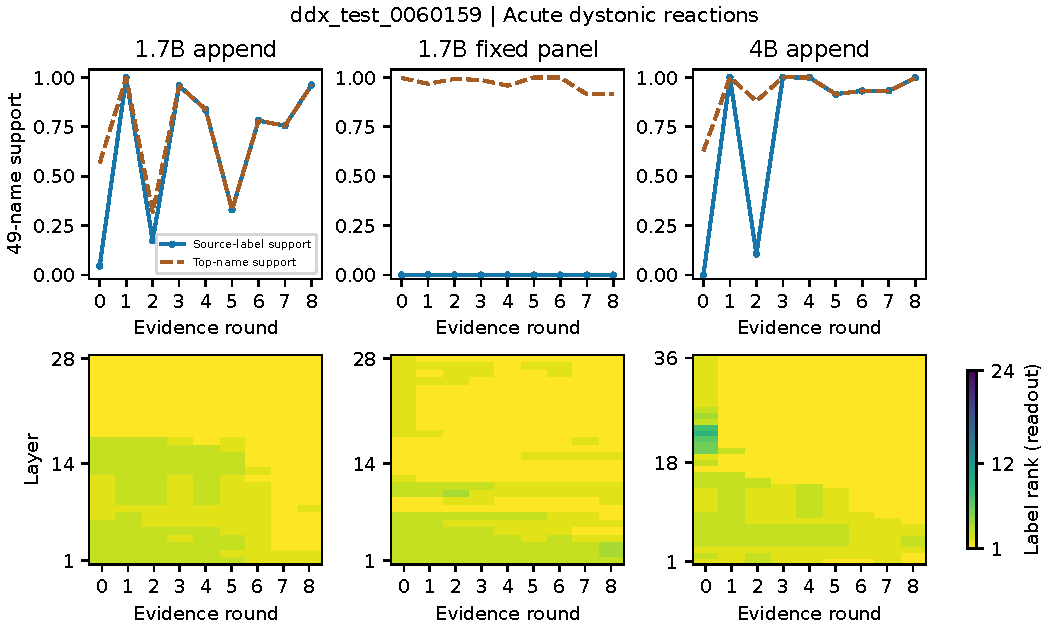
\includegraphics[width=.96\linewidth]{figures/ddx_test_0060159.pdf}\end{center}

{\small\begin{longtable}{>{\raggedright\arraybackslash}p{.07\textwidth}>{\raggedright\arraybackslash}p{.415\textwidth}>{\raggedright\arraybackslash}p{.415\textwidth}}\toprule Round & Newly revealed source evidence & Native top / label support / final-layer probe top \\ \midrule\endhead

0 & Do you feel that muscle spasms or soreness in your neck are keeping you from turning your head to one side? Yes & 1.7B append: Acute laryngitis / 0.0458 / Acute dystonic reactions\newline 1.7B panel: Acute COPD exacerbation / infection / 0.0001 / Myasthenia gravis\newline 4B append: Acute otitis media / 0.0000 / URTI \\ 

1 & Have you started or taken any antipsychotic medication within the last 7 days? Yes & 1.7B append: Acute dystonic reactions / 0.9990 / Acute dystonic reactions\newline 1.7B panel: Acute COPD exacerbation / infection / 0.0028 / Acute dystonic reactions\newline 4B append: Acute dystonic reactions / 1.0000 / Acute dystonic reactions \\ 

2 & Are you experiencing shortness of breath or difficulty breathing in a significant way? Yes & 1.7B append: Acute COPD exacerbation / infection / 0.1732 / Acute dystonic reactions\newline 1.7B panel: Acute pulmonary edema / 0.0000 / Acute dystonic reactions\newline 4B append: Acute pulmonary edema / 0.1068 / Acute dystonic reactions \\ 

3 & Do you have annoying muscle spasms in your face, neck or any other part of your body? Yes & 1.7B append: Acute dystonic reactions / 0.9577 / Acute dystonic reactions\newline 1.7B panel: Acute pulmonary edema / 0.0000 / Acute dystonic reactions\newline 4B append: Acute dystonic reactions / 0.9999 / Acute dystonic reactions \\ 

4 & Do you suddenly have difficulty or an inability to open your mouth or have jaw pain when opening it? Yes & 1.7B append: Acute dystonic reactions / 0.8381 / Acute dystonic reactions\newline 1.7B panel: Acute pulmonary edema / 0.0000 / Acute dystonic reactions\newline 4B append: Acute dystonic reactions / 0.9997 / Acute dystonic reactions \\ 

5 & Have you ever felt like you were suffocating for a very short time associated with inability to breathe or speak? Yes & 1.7B append: Acute dystonic reactions / 0.3305 / Acute dystonic reactions\newline 1.7B panel: Acute pulmonary edema / 0.0000 / Acute dystonic reactions\newline 4B append: Acute dystonic reactions / 0.9153 / Acute dystonic reactions \\ 

6 & Have you been treated in hospital recently for nausea, agitation, intoxication or aggressive behavior and received medication via an intravenous or intramuscular route? Yes & 1.7B append: Acute dystonic reactions / 0.7815 / Acute dystonic reactions\newline 1.7B panel: Acute pulmonary edema / 0.0000 / Acute dystonic reactions\newline 4B append: Acute dystonic reactions / 0.9318 / Acute dystonic reactions \\ 

7 & Do you regularly take stimulant drugs? Yes & 1.7B append: Acute dystonic reactions / 0.7554 / Acute dystonic reactions\newline 1.7B panel: Acute pulmonary edema / 0.0000 / Acute dystonic reactions\newline 4B append: Acute dystonic reactions / 0.9320 / Acute dystonic reactions \\ 

8 & Have you traveled out of the country in the last 4 weeks? No & 1.7B append: Acute dystonic reactions / 0.9620 / Acute dystonic reactions\newline 1.7B panel: Acute pulmonary edema / 0.0001 / Acute dystonic reactions\newline 4B append: Acute dystonic reactions / 0.9979 / Acute dystonic reactions \\ 

\bottomrule\end{longtable}}

\clearpage\subsection{ddx\_test\_0061730 -- Cluster headache}
\label{case:ddx_test_0061730}

Source label: Cluster headache. Family: neurologic. Evidence updates: 4. All facts below are source-recorded; their order is acquisition order.

\begin{center}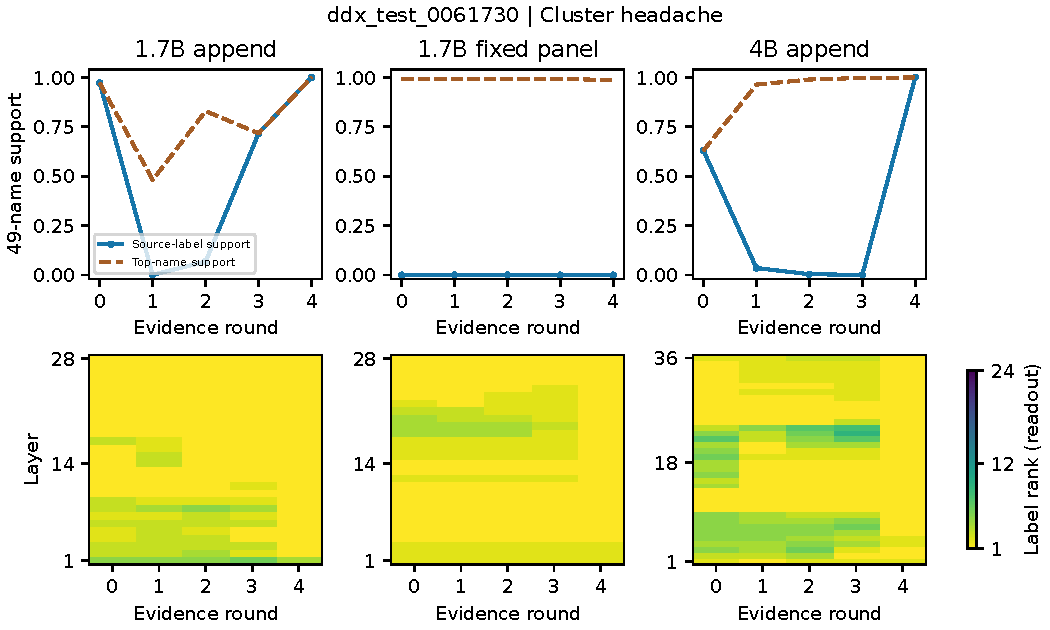
\includegraphics[width=.96\linewidth]{figures/ddx_test_0061730.pdf}\end{center}

{\small\begin{longtable}{>{\raggedright\arraybackslash}p{.07\textwidth}>{\raggedright\arraybackslash}p{.415\textwidth}>{\raggedright\arraybackslash}p{.415\textwidth}}\toprule Round & Newly revealed source evidence & Native top / label support / final-layer probe top \\ \midrule\endhead

0 & Do you have pain somewhere, related to your reason for consulting? Yes; Characterize your pain: haunting; a knife stroke; tugging; violent; sharp; Do you feel pain somewhere? forehead; cheek(R); cheek(L); eye(R); eye(L); How intense is the pain? Recorded scale value 9 on the dataset's 0-10 scale; endpoint meanings are unspecified; Does the pain radiate to another location? nowhere; How precisely is the pain located? Recorded scale value 10 on the dataset's 0-10 scale; endpoint meanings are unspecified; How fast did the pain appear? Recorded scale value 9 on the dataset's 0-10 scale; endpoint meanings are unspecified & 1.7B append: Cluster headache / 0.9719 / Cluster headache\newline 1.7B panel: Acute COPD exacerbation / infection / 0.0000 / Cluster headache\newline 4B append: Cluster headache / 0.6298 / SLE \\ 

1 & Do you drink alcohol excessively or do you have an addiction to alcohol? Yes & 1.7B append: Acute rhinosinusitis / 0.0010 / Cluster headache\newline 1.7B panel: Acute COPD exacerbation / infection / 0.0000 / Cluster headache\newline 4B append: Acute rhinosinusitis / 0.0357 / SLE \\ 

2 & Have you traveled out of the country in the last 4 weeks? No & 1.7B append: Acute rhinosinusitis / 0.0683 / Cluster headache\newline 1.7B panel: Acute COPD exacerbation / infection / 0.0000 / Cluster headache\newline 4B append: Acute rhinosinusitis / 0.0043 / SLE \\ 

3 & Do you take medication that dilates your blood vessels? Yes & 1.7B append: Cluster headache / 0.7170 / Cluster headache\newline 1.7B panel: Acute COPD exacerbation / infection / 0.0000 / Cluster headache\newline 4B append: Acute rhinosinusitis / 0.0010 / SLE \\ 

4 & Have any of your family members been diagnosed with cluster headaches? Yes & 1.7B append: Cluster headache / 1.0000 / Cluster headache\newline 1.7B panel: Acute COPD exacerbation / infection / 0.0000 / Cluster headache\newline 4B append: Cluster headache / 1.0000 / Cluster headache \\ 

\bottomrule\end{longtable}}

\clearpage\subsection{ddx\_test\_0062355 -- Acute dystonic reactions}
\label{case:ddx_test_0062355}

Source label: Acute dystonic reactions. Family: neurologic. Evidence updates: 8. All facts below are source-recorded; their order is acquisition order.

\begin{center}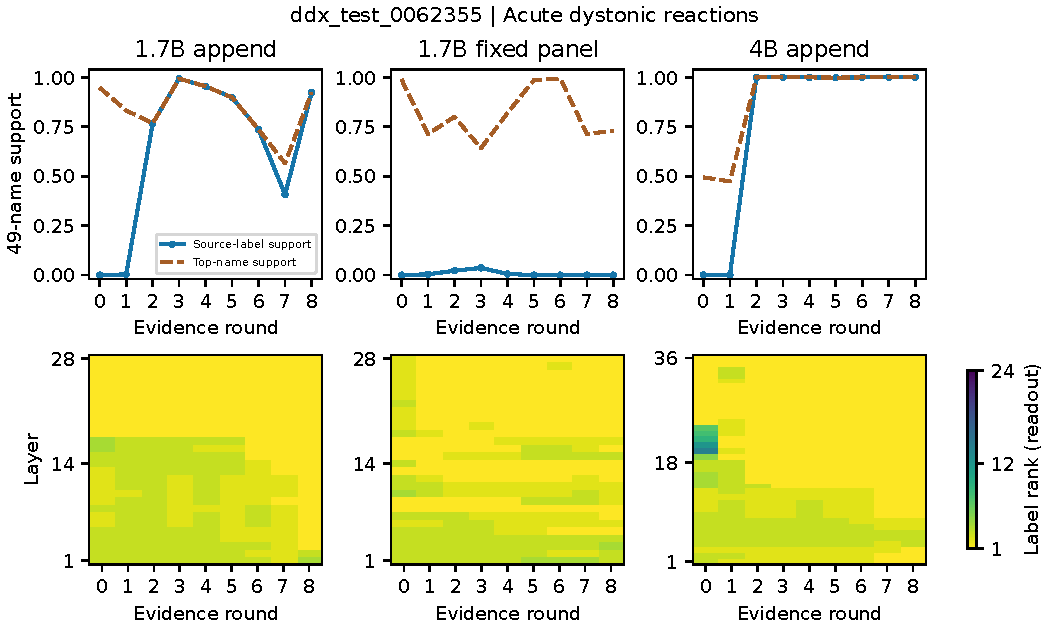
\includegraphics[width=.96\linewidth]{figures/ddx_test_0062355.pdf}\end{center}

{\small\begin{longtable}{>{\raggedright\arraybackslash}p{.07\textwidth}>{\raggedright\arraybackslash}p{.415\textwidth}>{\raggedright\arraybackslash}p{.415\textwidth}}\toprule Round & Newly revealed source evidence & Native top / label support / final-layer probe top \\ \midrule\endhead

0 & Are you unable to control the direction of your eyes? Yes & 1.7B append: Acute COPD exacerbation / infection / 0.0001 / Acute dystonic reactions\newline 1.7B panel: Acute COPD exacerbation / infection / 0.0000 / Myasthenia gravis\newline 4B append: Acute rhinosinusitis / 0.0012 / Acute dystonic reactions \\ 

1 & Do you suddenly have difficulty or an inability to open your mouth or have jaw pain when opening it? Yes & 1.7B append: Acute laryngitis / 0.0034 / Acute dystonic reactions\newline 1.7B panel: Acute COPD exacerbation / infection / 0.0037 / Acute dystonic reactions\newline 4B append: Acute rhinosinusitis / 0.0000 / Acute dystonic reactions \\ 

2 & Have you started or taken any antipsychotic medication within the last 7 days? Yes & 1.7B append: Acute dystonic reactions / 0.7669 / Acute dystonic reactions\newline 1.7B panel: Acute laryngitis / 0.0220 / Acute dystonic reactions\newline 4B append: Acute dystonic reactions / 1.0000 / Acute dystonic reactions \\ 

3 & Have you traveled out of the country in the last 4 weeks? No & 1.7B append: Acute dystonic reactions / 0.9938 / Acute dystonic reactions\newline 1.7B panel: Acute laryngitis / 0.0362 / Acute dystonic reactions\newline 4B append: Acute dystonic reactions / 1.0000 / Acute dystonic reactions \\ 

4 & Have you been treated in hospital recently for nausea, agitation, intoxication or aggressive behavior and received medication via an intravenous or intramuscular route? Yes & 1.7B append: Acute dystonic reactions / 0.9547 / Acute dystonic reactions\newline 1.7B panel: Acute COPD exacerbation / infection / 0.0054 / Acute dystonic reactions\newline 4B append: Acute dystonic reactions / 1.0000 / Acute dystonic reactions \\ 

5 & Are you experiencing shortness of breath or difficulty breathing in a significant way? Yes & 1.7B append: Acute dystonic reactions / 0.8985 / Acute dystonic reactions\newline 1.7B panel: Acute pulmonary edema / 0.0000 / Acute dystonic reactions\newline 4B append: Acute dystonic reactions / 0.9990 / Acute dystonic reactions \\ 

6 & Do you have a hard time opening/raising one or both eyelids? Yes & 1.7B append: Acute dystonic reactions / 0.7363 / Acute dystonic reactions\newline 1.7B panel: Acute pulmonary edema / 0.0000 / Acute dystonic reactions\newline 4B append: Acute dystonic reactions / 1.0000 / Acute dystonic reactions \\ 

7 & Do you regularly take stimulant drugs? Yes & 1.7B append: Acute laryngitis / 0.4070 / Acute dystonic reactions\newline 1.7B panel: Acute pulmonary edema / 0.0002 / Acute dystonic reactions\newline 4B append: Acute dystonic reactions / 1.0000 / Acute dystonic reactions \\ 

8 & Do you feel that muscle spasms or soreness in your neck are keeping you from turning your head to one side? Yes & 1.7B append: Acute dystonic reactions / 0.9228 / Acute dystonic reactions\newline 1.7B panel: Acute pulmonary edema / 0.0001 / Acute dystonic reactions\newline 4B append: Acute dystonic reactions / 1.0000 / Acute dystonic reactions \\ 

\bottomrule\end{longtable}}

\clearpage\subsection{ddx\_test\_0064225 -- Acute pulmonary edema}
\label{case:ddx_test_0064225}

Source label: Acute pulmonary edema. Family: respiratory. Evidence updates: 12. All facts below are source-recorded; their order is acquisition order.

\begin{center}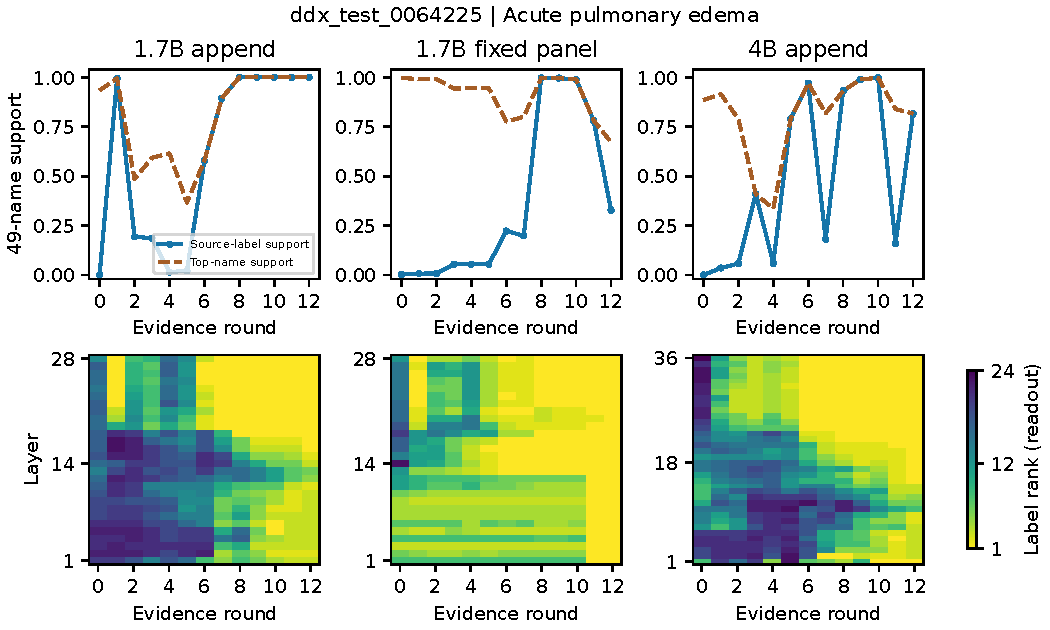
\includegraphics[width=.96\linewidth]{figures/ddx_test_0064225.pdf}\end{center}

{\small\begin{longtable}{>{\raggedright\arraybackslash}p{.07\textwidth}>{\raggedright\arraybackslash}p{.415\textwidth}>{\raggedright\arraybackslash}p{.415\textwidth}}\toprule Round & Newly revealed source evidence & Native top / label support / final-layer probe top \\ \midrule\endhead

0 & Do you have pain somewhere, related to your reason for consulting? Yes; Characterize your pain: sensitive; Do you feel pain somewhere? lower chest; ankle(R); ankle(L); side of the chest(L); breast(R); How intense is the pain? Recorded scale value 2 on the dataset's 0-10 scale; endpoint meanings are unspecified; Does the pain radiate to another location? biceps(R); biceps(L); chin; jaw; shoulder(R); How precisely is the pain located? Recorded scale value 7 on the dataset's 0-10 scale; endpoint meanings are unspecified; How fast did the pain appear? Recorded scale value 1 on the dataset's 0-10 scale; endpoint meanings are unspecified & 1.7B append: Acute rhinosinusitis / 0.0020 / Inguinal hernia\newline 1.7B panel: Acute COPD exacerbation / infection / 0.0027 / Pericarditis\newline 4B append: Acute rhinosinusitis / 0.0001 / Possible NSTEMI / STEMI \\ 

1 & Have you ever had fluid in your lungs? Yes & 1.7B append: Acute pulmonary edema / 0.9951 / Acute pulmonary edema\newline 1.7B panel: Acute COPD exacerbation / infection / 0.0075 / Acute pulmonary edema\newline 4B append: Pneumonia / 0.0356 / Pericarditis \\ 

2 & Do you have symptoms that are increased with physical exertion but alleviated with rest? Yes & 1.7B append: Acute rhinosinusitis / 0.1935 / Bronchitis\newline 1.7B panel: Acute COPD exacerbation / infection / 0.0081 / Stable angina\newline 4B append: Pneumonia / 0.0586 / Pericarditis \\ 

3 & Do you have bouts of choking or shortness of breath that wake you up at night? Yes & 1.7B append: Acute laryngitis / 0.1867 / Bronchitis\newline 1.7B panel: Acute COPD exacerbation / infection / 0.0549 / Stable angina\newline 4B append: Acute pulmonary edema / 0.4096 / Bronchitis \\ 

4 & Have you traveled out of the country in the last 4 weeks? No & 1.7B append: Acute laryngitis / 0.0149 / Bronchitis\newline 1.7B panel: Acute COPD exacerbation / infection / 0.0541 / Stable angina\newline 4B append: Pneumonia / 0.0588 / Bronchitis \\ 

5 & Are your symptoms worse when lying down and alleviated while sitting up? Yes & 1.7B append: Acute laryngitis / 0.0220 / Bronchitis\newline 1.7B panel: Acute COPD exacerbation / infection / 0.0542 / Guillain-Barr\'{e} syndrome\newline 4B append: Acute pulmonary edema / 0.7905 / Bronchitis \\ 

6 & Do you currently undergo dialysis? Yes & 1.7B append: Acute pulmonary edema / 0.5785 / Bronchitis\newline 1.7B panel: Acute COPD exacerbation / infection / 0.2226 / Acute pulmonary edema\newline 4B append: Acute pulmonary edema / 0.9707 / Acute pulmonary edema \\ 

7 & Are you experiencing shortness of breath or difficulty breathing in a significant way? Yes & 1.7B append: Acute pulmonary edema / 0.8950 / Acute pulmonary edema\newline 1.7B panel: Acute COPD exacerbation / infection / 0.1992 / Guillain-Barr\'{e} syndrome\newline 4B append: Pulmonary embolism / 0.1806 / Acute pulmonary edema \\ 

8 & Do you have heart failure? Yes & 1.7B append: Acute pulmonary edema / 1.0000 / Acute pulmonary edema\newline 1.7B panel: Acute pulmonary edema / 0.9974 / Acute pulmonary edema\newline 4B append: Acute pulmonary edema / 0.9318 / Acute pulmonary edema \\ 

9 & Have you had significantly increased sweating? Yes & 1.7B append: Acute pulmonary edema / 1.0000 / Acute pulmonary edema\newline 1.7B panel: Acute pulmonary edema / 0.9966 / Acute pulmonary edema\newline 4B append: Acute pulmonary edema / 0.9906 / Acute pulmonary edema \\ 

10 & Do you have high blood pressure or do you take medications to treat high blood pressure? Yes & 1.7B append: Acute pulmonary edema / 1.0000 / Acute pulmonary edema\newline 1.7B panel: Acute pulmonary edema / 0.9893 / Acute pulmonary edema\newline 4B append: Acute pulmonary edema / 0.9976 / Acute pulmonary edema \\ 

11 & Do you have swelling in one or more areas of your body? Yes; Where is the swelling located? ankle(R); calf(R); calf(L); tibia(L) & 1.7B append: Acute pulmonary edema / 1.0000 / Acute pulmonary edema\newline 1.7B panel: Acute pulmonary edema / 0.7826 / Acute pulmonary edema\newline 4B append: Pulmonary embolism / 0.1604 / Acute pulmonary edema \\ 

12 & Have you ever had a heart attack or do you have angina (chest pain)? Yes & 1.7B append: Acute pulmonary edema / 1.0000 / Acute pulmonary edema\newline 1.7B panel: Acute COPD exacerbation / infection / 0.3277 / Acute pulmonary edema\newline 4B append: Acute pulmonary edema / 0.8167 / Acute pulmonary edema \\ 

\bottomrule\end{longtable}}

\clearpage\subsection{ddx\_test\_0067994 -- Bronchitis}
\label{case:ddx_test_0067994}

Source label: Bronchitis. Family: respiratory. Evidence updates: 9. All facts below are source-recorded; their order is acquisition order.

\begin{center}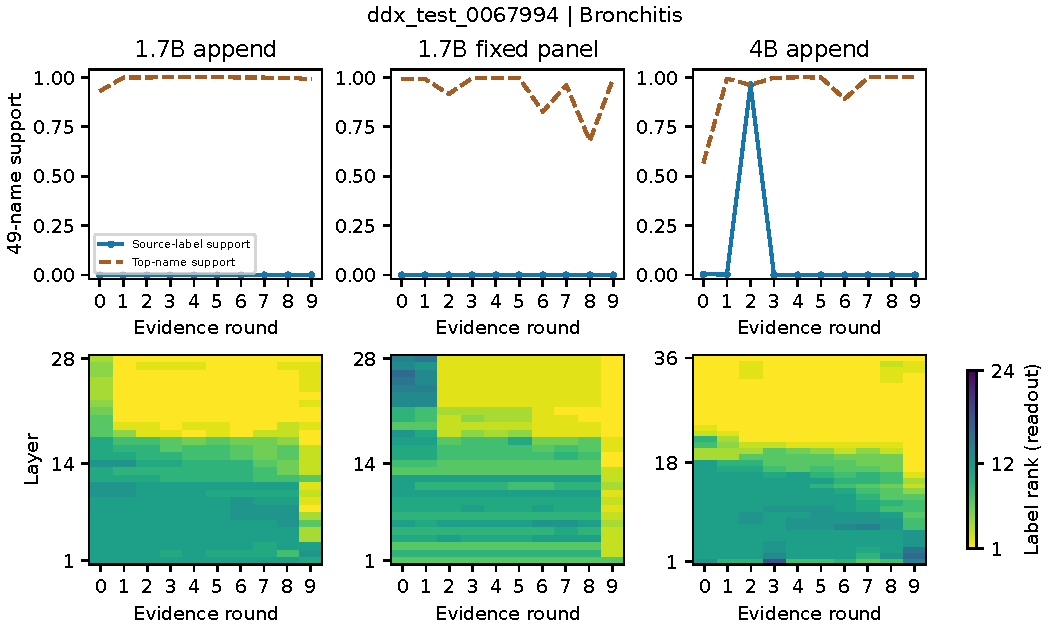
\includegraphics[width=.96\linewidth]{figures/ddx_test_0067994.pdf}\end{center}

{\small\begin{longtable}{>{\raggedright\arraybackslash}p{.07\textwidth}>{\raggedright\arraybackslash}p{.415\textwidth}>{\raggedright\arraybackslash}p{.415\textwidth}}\toprule Round & Newly revealed source evidence & Native top / label support / final-layer probe top \\ \midrule\endhead

0 & Are you experiencing shortness of breath or difficulty breathing in a significant way? Yes & 1.7B append: Acute pulmonary edema / 0.0000 / Acute pulmonary edema\newline 1.7B panel: Acute pulmonary edema / 0.0000 / Guillain-Barr\'{e} syndrome\newline 4B append: Acute COPD exacerbation / infection / 0.0039 / Bronchitis \\ 

1 & Do you smoke cigarettes? Yes & 1.7B append: Acute COPD exacerbation / infection / 0.0000 / Bronchitis\newline 1.7B panel: Acute pulmonary edema / 0.0000 / Guillain-Barr\'{e} syndrome\newline 4B append: Acute COPD exacerbation / infection / 0.0026 / Bronchitis \\ 

2 & Have you noticed a wheezing sound when you exhale? Yes & 1.7B append: Acute COPD exacerbation / infection / 0.0000 / Bronchitis\newline 1.7B panel: Acute pulmonary edema / 0.0000 / Bronchospasm / acute asthma exacerbation\newline 4B append: Bronchitis / 0.9620 / Bronchitis \\ 

3 & Do you have a fever (either felt or measured with a thermometer)? Yes & 1.7B append: Acute COPD exacerbation / infection / 0.0000 / Bronchitis\newline 1.7B panel: Acute pulmonary edema / 0.0000 / Bronchospasm / acute asthma exacerbation\newline 4B append: Acute COPD exacerbation / infection / 0.0000 / Bronchitis \\ 

4 & Are your symptoms more prominent at night? Yes & 1.7B append: Acute COPD exacerbation / infection / 0.0000 / Bronchitis\newline 1.7B panel: Acute pulmonary edema / 0.0000 / Bronchospasm / acute asthma exacerbation\newline 4B append: Acute COPD exacerbation / infection / 0.0000 / Bronchitis \\ 

5 & Have you traveled out of the country in the last 4 weeks? No & 1.7B append: Acute COPD exacerbation / infection / 0.0000 / Bronchitis\newline 1.7B panel: Acute pulmonary edema / 0.0000 / Bronchospasm / acute asthma exacerbation\newline 4B append: Acute COPD exacerbation / infection / 0.0000 / Bronchitis \\ 

6 & Do you have a cough? Yes & 1.7B append: Acute COPD exacerbation / infection / 0.0000 / Bronchitis\newline 1.7B panel: Acute pulmonary edema / 0.0000 / Bronchospasm / acute asthma exacerbation\newline 4B append: Pneumonia / 0.0000 / Bronchitis \\ 

7 & Do you have a cough that produces colored or more abundant sputum than usual? Yes & 1.7B append: Acute COPD exacerbation / infection / 0.0000 / Bronchitis\newline 1.7B panel: Acute pulmonary edema / 0.0000 / Bronchospasm / acute asthma exacerbation\newline 4B append: Pneumonia / 0.0000 / Bronchitis \\ 

8 & Do you have a chronic obstructive pulmonary disease (COPD)? Yes & 1.7B append: Acute COPD exacerbation / infection / 0.0000 / Bronchitis\newline 1.7B panel: Acute COPD exacerbation / infection / 0.0000 / Bronchospasm / acute asthma exacerbation\newline 4B append: Acute COPD exacerbation / infection / 0.0000 / Bronchitis \\ 

9 & Do you have pain somewhere, related to your reason for consulting? Yes; Characterize your pain: sensitive; burning; Do you feel pain somewhere? breast(R); posterior chest wall(R); posterior chest wall(L); How intense is the pain? Recorded scale value 2 on the dataset's 0-10 scale; endpoint meanings are unspecified; Does the pain radiate to another location? nowhere; How precisely is the pain located? Recorded scale value 5 on the dataset's 0-10 scale; endpoint meanings are unspecified; How fast did the pain appear? Recorded scale value 1 on the dataset's 0-10 scale; endpoint meanings are unspecified & 1.7B append: Acute COPD exacerbation / infection / 0.0000 / Bronchitis\newline 1.7B panel: Acute COPD exacerbation / infection / 0.0000 / Bronchitis\newline 4B append: Acute COPD exacerbation / infection / 0.0000 / Bronchitis \\ 

\bottomrule\end{longtable}}

\clearpage\subsection{ddx\_test\_0077278 -- Pericarditis}
\label{case:ddx_test_0077278}

Source label: Pericarditis. Family: cardiovascular. Evidence updates: 7. All facts below are source-recorded; their order is acquisition order.

\begin{center}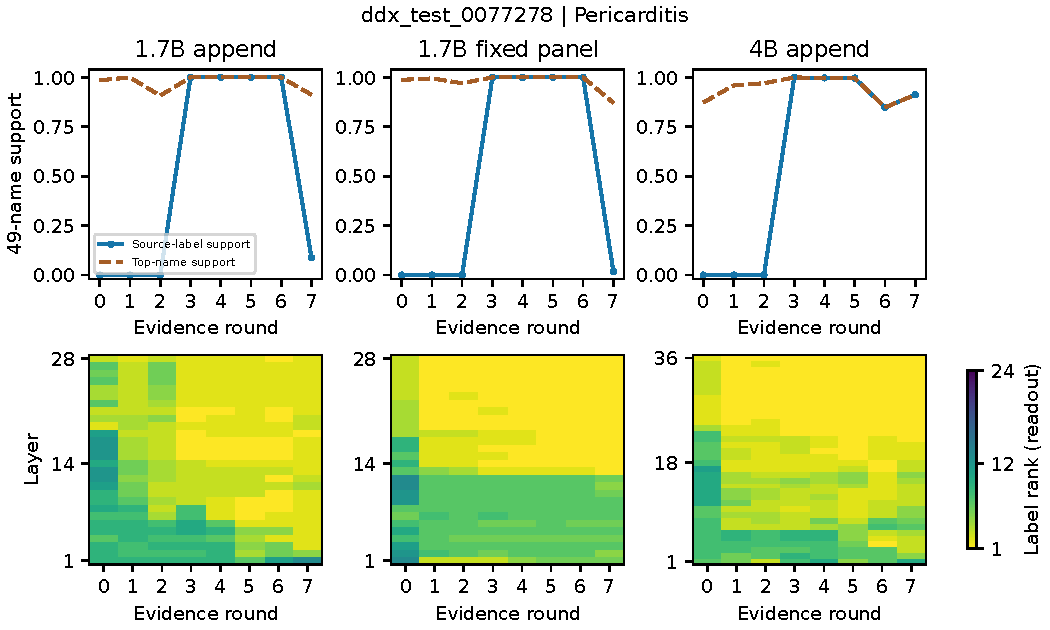
\includegraphics[width=.96\linewidth]{figures/ddx_test_0077278.pdf}\end{center}

{\small\begin{longtable}{>{\raggedright\arraybackslash}p{.07\textwidth}>{\raggedright\arraybackslash}p{.415\textwidth}>{\raggedright\arraybackslash}p{.415\textwidth}}\toprule Round & Newly revealed source evidence & Native top / label support / final-layer probe top \\ \midrule\endhead

0 & Are you experiencing shortness of breath or difficulty breathing in a significant way? Yes & 1.7B append: Acute COPD exacerbation / infection / 0.0000 / Bronchitis\newline 1.7B panel: Acute pulmonary edema / 0.0000 / Guillain-Barr\'{e} syndrome\newline 4B append: Bronchitis / 0.0000 / Bronchitis \\ 

1 & Do you have pain somewhere, related to your reason for consulting? Yes; Characterize your pain: a knife stroke; sharp; Do you feel pain somewhere? lower chest; breast(R); How intense is the pain? Recorded scale value 8 on the dataset's 0-10 scale; endpoint meanings are unspecified; Does the pain radiate to another location? nowhere; How precisely is the pain located? Recorded scale value 7 on the dataset's 0-10 scale; endpoint meanings are unspecified; How fast did the pain appear? Recorded scale value 7 on the dataset's 0-10 scale; endpoint meanings are unspecified & 1.7B append: Boerhaave / 0.0000 / Pulmonary embolism\newline 1.7B panel: Acute COPD exacerbation / infection / 0.0000 / Pericarditis\newline 4B append: Bronchospasm / acute asthma exacerbation / 0.0000 / Pericarditis \\ 

2 & Do you have pain that is increased when you breathe in deeply? Yes & 1.7B append: Bronchospasm / acute asthma exacerbation / 0.0000 / Acute dystonic reactions\newline 1.7B panel: Acute COPD exacerbation / infection / 0.0000 / Pericarditis\newline 4B append: Bronchospasm / acute asthma exacerbation / 0.0000 / Pericarditis \\ 

3 & Have you ever had a pericarditis? Yes & 1.7B append: Pericarditis / 1.0000 / SLE\newline 1.7B panel: Pericarditis / 1.0000 / Pericarditis\newline 4B append: Pericarditis / 0.9998 / Pericarditis \\ 

4 & Have you traveled out of the country in the last 4 weeks? No & 1.7B append: Pericarditis / 1.0000 / SLE\newline 1.7B panel: Pericarditis / 1.0000 / Pericarditis\newline 4B append: Pericarditis / 0.9974 / Pericarditis \\ 

5 & Do you feel your heart is beating fast (racing), irregularly (missing a beat) or do you feel palpitations? Yes & 1.7B append: Pericarditis / 0.9999 / SLE\newline 1.7B panel: Pericarditis / 1.0000 / Pericarditis\newline 4B append: Pericarditis / 0.9966 / Pericarditis \\ 

6 & Are your symptoms worse when lying down and alleviated while sitting up? Yes & 1.7B append: Pericarditis / 1.0000 / Pericarditis\newline 1.7B panel: Pericarditis / 1.0000 / Pericarditis\newline 4B append: Pericarditis / 0.8480 / Pericarditis \\ 

7 & Have you recently had a viral infection? Yes & 1.7B append: Boerhaave / 0.0876 / Pulmonary embolism\newline 1.7B panel: Acute COPD exacerbation / infection / 0.0179 / Pericarditis\newline 4B append: Pericarditis / 0.9124 / Pericarditis \\ 

\bottomrule\end{longtable}}

\clearpage\subsection{ddx\_test\_0079685 -- Guillain-Barr\'{e} syndrome}
\label{case:ddx_test_0079685}

Source label: Guillain-Barr\'{e} syndrome. Family: neurologic. Evidence updates: 7. All facts below are source-recorded; their order is acquisition order.

\begin{center}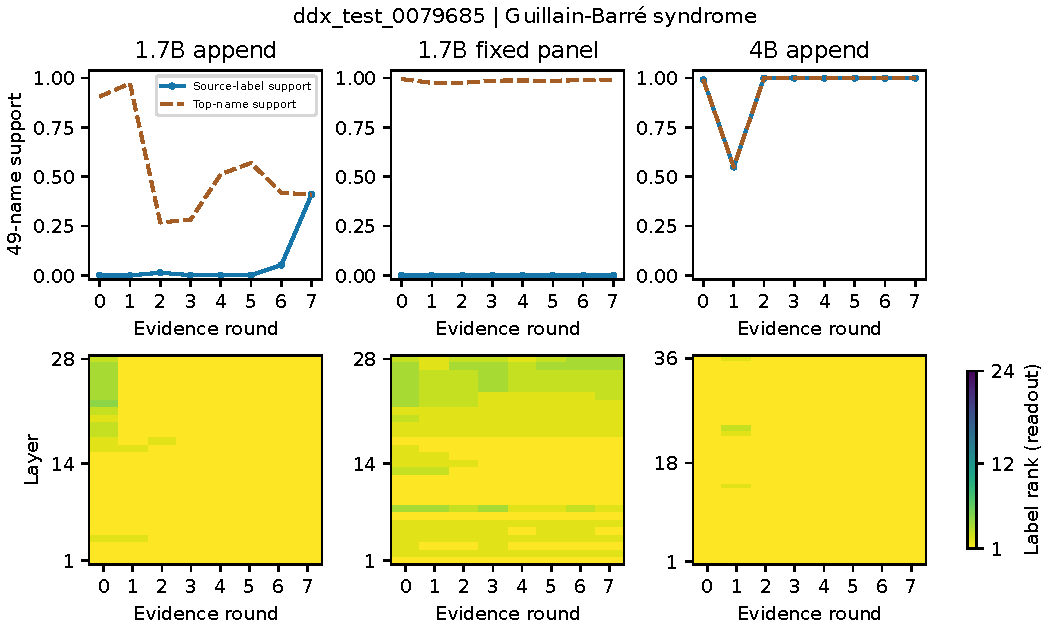
\includegraphics[width=.96\linewidth]{figures/ddx_test_0079685.pdf}\end{center}

{\small\begin{longtable}{>{\raggedright\arraybackslash}p{.07\textwidth}>{\raggedright\arraybackslash}p{.415\textwidth}>{\raggedright\arraybackslash}p{.415\textwidth}}\toprule Round & Newly revealed source evidence & Native top / label support / final-layer probe top \\ \midrule\endhead

0 & Have you had weakness or paralysis on one side of the face, which may still be present or completely resolved? Yes & 1.7B append: Acute COPD exacerbation / infection / 0.0000 / Bronchitis\newline 1.7B panel: Acute COPD exacerbation / infection / 0.0000 / Myasthenia gravis\newline 4B append: Guillain-Barr\'{e} syndrome / 0.9914 / Guillain-Barr\'{e} syndrome \\ 

1 & Do you have numbness, loss of sensation or tingling in the feet? Yes & 1.7B append: Acute rhinosinusitis / 0.0000 / Guillain-Barr\'{e} syndrome\newline 1.7B panel: Acute COPD exacerbation / infection / 0.0000 / Myasthenia gravis\newline 4B append: Guillain-Barr\'{e} syndrome / 0.5498 / Myasthenia gravis \\ 

2 & Did you previously, or do you currently, have any weakness/paralysis in one or more of your limbs or in your face? Yes & 1.7B append: Acute rhinosinusitis / 0.0139 / Guillain-Barr\'{e} syndrome\newline 1.7B panel: Acute COPD exacerbation / infection / 0.0000 / Myasthenia gravis\newline 4B append: Guillain-Barr\'{e} syndrome / 1.0000 / Guillain-Barr\'{e} syndrome \\ 

3 & Do you feel weakness in both arms and/or both legs? Yes & 1.7B append: Myasthenia gravis / 0.0015 / Guillain-Barr\'{e} syndrome\newline 1.7B panel: Acute COPD exacerbation / infection / 0.0000 / Myasthenia gravis\newline 4B append: Guillain-Barr\'{e} syndrome / 1.0000 / Guillain-Barr\'{e} syndrome \\ 

4 & Have you recently had a viral infection? Yes & 1.7B append: Acute rhinosinusitis / 0.0000 / Guillain-Barr\'{e} syndrome\newline 1.7B panel: Acute COPD exacerbation / infection / 0.0000 / Myasthenia gravis\newline 4B append: Guillain-Barr\'{e} syndrome / 1.0000 / Guillain-Barr\'{e} syndrome \\ 

5 & Have you recently had numbness, loss of sensation or tingling, in both arms and legs and around your mouth? Yes & 1.7B append: Acute rhinosinusitis / 0.0008 / Guillain-Barr\'{e} syndrome\newline 1.7B panel: Acute COPD exacerbation / infection / 0.0000 / Myasthenia gravis\newline 4B append: Guillain-Barr\'{e} syndrome / 1.0000 / Guillain-Barr\'{e} syndrome \\ 

6 & Have you traveled out of the country in the last 4 weeks? No & 1.7B append: Acute COPD exacerbation / infection / 0.0526 / Guillain-Barr\'{e} syndrome\newline 1.7B panel: Acute COPD exacerbation / infection / 0.0000 / Myasthenia gravis\newline 4B append: Guillain-Barr\'{e} syndrome / 1.0000 / Guillain-Barr\'{e} syndrome \\ 

7 & Do you currently, or did you ever, have numbness, loss of sensitivity or tingling anywhere on your body? Yes & 1.7B append: Guillain-Barr\'{e} syndrome / 0.4097 / Guillain-Barr\'{e} syndrome\newline 1.7B panel: Acute COPD exacerbation / infection / 0.0000 / Myasthenia gravis\newline 4B append: Guillain-Barr\'{e} syndrome / 1.0000 / Guillain-Barr\'{e} syndrome \\ 

\bottomrule\end{longtable}}

\clearpage\subsection{ddx\_test\_0084538 -- Inguinal hernia}
\label{case:ddx_test_0084538}

Source label: Inguinal hernia. Family: digestive. Evidence updates: 8. All facts below are source-recorded; their order is acquisition order.

\begin{center}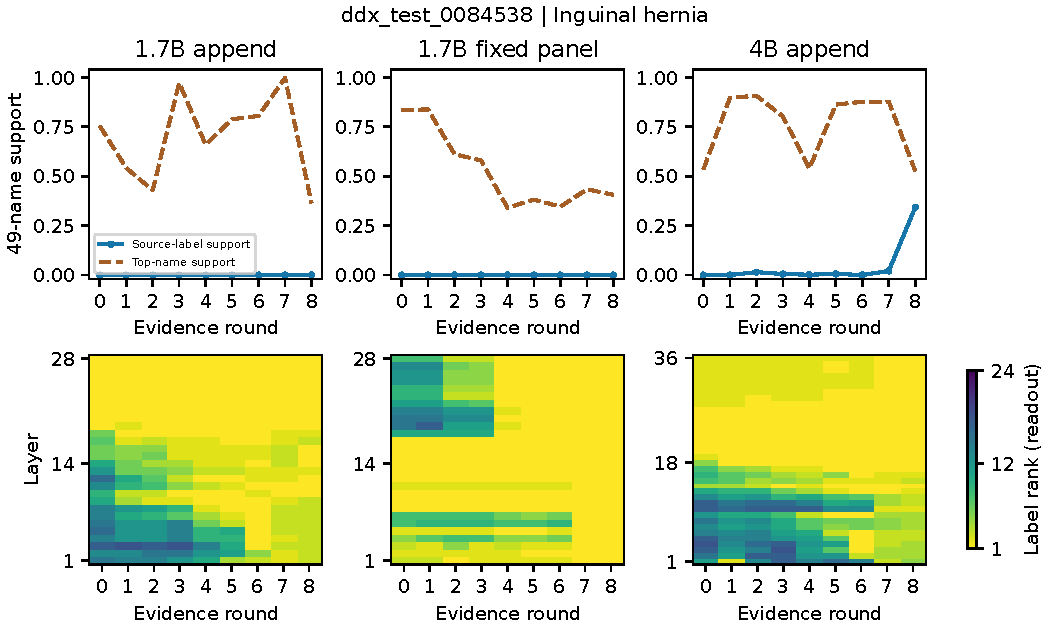
\includegraphics[width=.96\linewidth]{figures/ddx_test_0084538.pdf}\end{center}

{\small\begin{longtable}{>{\raggedright\arraybackslash}p{.07\textwidth}>{\raggedright\arraybackslash}p{.415\textwidth}>{\raggedright\arraybackslash}p{.415\textwidth}}\toprule Round & Newly revealed source evidence & Native top / label support / final-layer probe top \\ \midrule\endhead

0 & Do you have any lesions, redness or problems on your skin that you believe are related to the condition you are consulting for? Yes; What color is the rash? pale; Do your lesions peel off? No; Is the rash swollen? Recorded scale value 4 on the dataset's 0-10 scale; endpoint meanings are unspecified; Where is the affected region located? iliac fossa(R); iliac fossa(L); How intense is the pain caused by the rash? Recorded scale value 6 on the dataset's 0-10 scale; endpoint meanings are unspecified; Is the lesion (or are the lesions) larger than 1cm? Yes; How severe is the itching? Recorded scale value 0 on the dataset's 0-10 scale; endpoint meanings are unspecified & 1.7B append: Localized edema / 0.0001 / Inguinal hernia\newline 1.7B panel: Acute COPD exacerbation / infection / 0.0000 / Myasthenia gravis\newline 4B append: Pulmonary embolism / 0.0000 / SLE \\ 

1 & Were you born prematurely or did you suffer any complication at birth? Yes & 1.7B append: Acute rhinosinusitis / 0.0000 / Inguinal hernia\newline 1.7B panel: Acute COPD exacerbation / infection / 0.0000 / Myasthenia gravis\newline 4B append: Pulmonary embolism / 0.0003 / SLE \\ 

2 & Do you feel your abdomen is bloated or distended (swollen due to pressure from inside)? Yes & 1.7B append: Acute pulmonary edema / 0.0001 / Inguinal hernia\newline 1.7B panel: Acute COPD exacerbation / infection / 0.0000 / HIV (initial infection)\newline 4B append: Pulmonary embolism / 0.0148 / SLE \\ 

3 & Have you been able to pass stools or gas since your symptoms increased? Yes & 1.7B append: Localized edema / 0.0000 / Inguinal hernia\newline 1.7B panel: Acute COPD exacerbation / infection / 0.0000 / HIV (initial infection)\newline 4B append: Pulmonary embolism / 0.0053 / SLE \\ 

4 & Do you have intense coughing fits? Yes & 1.7B append: Pneumonia / 0.0000 / Inguinal hernia\newline 1.7B panel: Acute pulmonary edema / 0.0000 / Inguinal hernia\newline 4B append: Pulmonary embolism / 0.0018 / SLE \\ 

5 & Are the symptoms or pain increased with coughing, with an effort like lifting a weight or from forcing a bowel movement? Yes & 1.7B append: Pneumonia / 0.0000 / Inguinal hernia\newline 1.7B panel: Acute pulmonary edema / 0.0000 / Inguinal hernia\newline 4B append: Pneumonia / 0.0059 / SLE \\ 

6 & Have you traveled out of the country in the last 4 weeks? No & 1.7B append: Pneumonia / 0.0000 / Inguinal hernia\newline 1.7B panel: Acute pulmonary edema / 0.0000 / Inguinal hernia\newline 4B append: Pneumonia / 0.0003 / SLE \\ 

7 & Do you have pain somewhere, related to your reason for consulting? Yes; Characterize your pain: heavy; Do you feel pain somewhere? iliac fossa(R); iliac fossa(L); hip(R); hip(L); How intense is the pain? Recorded scale value 3 on the dataset's 0-10 scale; endpoint meanings are unspecified; Does the pain radiate to another location? nowhere; How precisely is the pain located? Recorded scale value 0 on the dataset's 0-10 scale; endpoint meanings are unspecified; How fast did the pain appear? Recorded scale value 1 on the dataset's 0-10 scale; endpoint meanings are unspecified & 1.7B append: Localized edema / 0.0000 / Inguinal hernia\newline 1.7B panel: Acute pulmonary edema / 0.0000 / Inguinal hernia\newline 4B append: Pneumonia / 0.0207 / Inguinal hernia \\ 

8 & Are you significantly overweight compared to people of the same height as you? Yes & 1.7B append: Localized edema / 0.0000 / Inguinal hernia\newline 1.7B panel: Acute pulmonary edema / 0.0000 / Inguinal hernia\newline 4B append: Pneumonia / 0.3426 / Inguinal hernia \\ 

\bottomrule\end{longtable}}

\clearpage\subsection{ddx\_test\_0101113 -- Spontaneous pneumothorax}
\label{case:ddx_test_0101113}

Source label: Spontaneous pneumothorax. Family: respiratory. Evidence updates: 5. All facts below are source-recorded; their order is acquisition order.

\begin{center}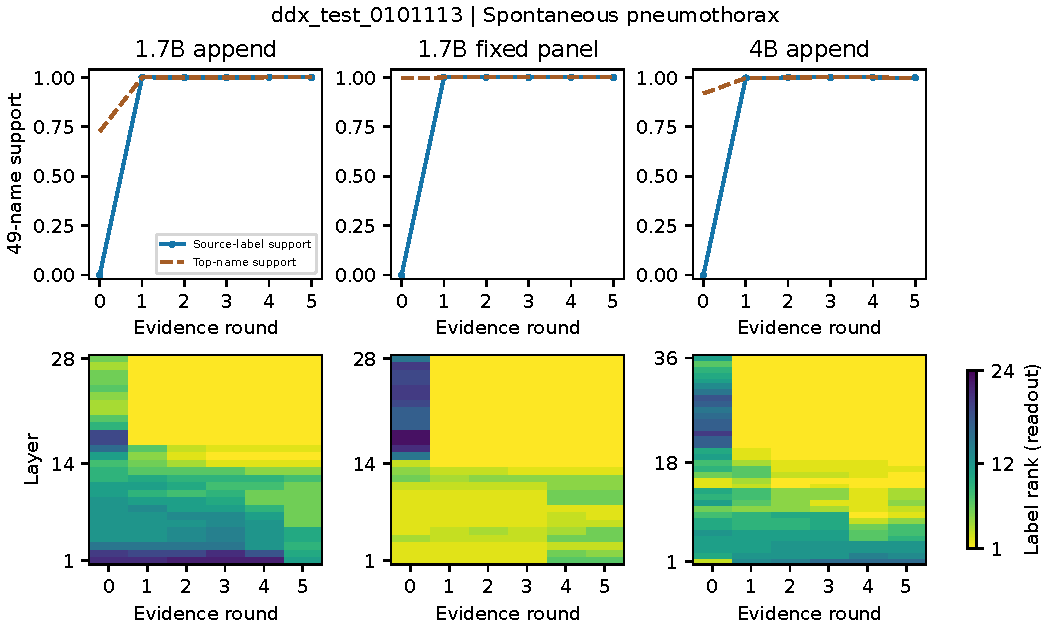
\includegraphics[width=.96\linewidth]{figures/ddx_test_0101113.pdf}\end{center}

{\small\begin{longtable}{>{\raggedright\arraybackslash}p{.07\textwidth}>{\raggedright\arraybackslash}p{.415\textwidth}>{\raggedright\arraybackslash}p{.415\textwidth}}\toprule Round & Newly revealed source evidence & Native top / label support / final-layer probe top \\ \midrule\endhead

0 & Do you have pain somewhere, related to your reason for consulting? Yes; Characterize your pain: heartbreaking; a knife stroke; Do you feel pain somewhere? lower chest; side of the chest(R); upper chest; breast(R); breast(L); How intense is the pain? Recorded scale value 7 on the dataset's 0-10 scale; endpoint meanings are unspecified; Does the pain radiate to another location? nowhere; How precisely is the pain located? Recorded scale value 6 on the dataset's 0-10 scale; endpoint meanings are unspecified; How fast did the pain appear? Recorded scale value 6 on the dataset's 0-10 scale; endpoint meanings are unspecified & 1.7B append: Acute pulmonary edema / 0.0001 / Pericarditis\newline 1.7B panel: Acute COPD exacerbation / infection / 0.0000 / Boerhaave\newline 4B append: Pericarditis / 0.0000 / Pericarditis \\ 

1 & Have you ever had a spontaneous pneumothorax? Yes & 1.7B append: Spontaneous pneumothorax / 1.0000 / Spontaneous pneumothorax\newline 1.7B panel: Spontaneous pneumothorax / 1.0000 / Spontaneous pneumothorax\newline 4B append: Spontaneous pneumothorax / 0.9969 / Spontaneous pneumothorax \\ 

2 & Do you have pain that is increased when you breathe in deeply? Yes & 1.7B append: Spontaneous pneumothorax / 0.9994 / Spontaneous pneumothorax\newline 1.7B panel: Spontaneous pneumothorax / 1.0000 / Spontaneous pneumothorax\newline 4B append: Spontaneous pneumothorax / 0.9997 / Spontaneous pneumothorax \\ 

3 & Do you smoke cigarettes? Yes & 1.7B append: Spontaneous pneumothorax / 0.9994 / Spontaneous pneumothorax\newline 1.7B panel: Spontaneous pneumothorax / 1.0000 / Spontaneous pneumothorax\newline 4B append: Spontaneous pneumothorax / 1.0000 / Spontaneous pneumothorax \\ 

4 & Have you traveled out of the country in the last 4 weeks? North America & 1.7B append: Spontaneous pneumothorax / 0.9999 / Spontaneous pneumothorax\newline 1.7B panel: Spontaneous pneumothorax / 1.0000 / Spontaneous pneumothorax\newline 4B append: Spontaneous pneumothorax / 1.0000 / Spontaneous pneumothorax \\ 

5 & Do you have symptoms that are increased with physical exertion but alleviated with rest? Yes & 1.7B append: Spontaneous pneumothorax / 1.0000 / Spontaneous pneumothorax\newline 1.7B panel: Spontaneous pneumothorax / 1.0000 / Spontaneous pneumothorax\newline 4B append: Spontaneous pneumothorax / 0.9979 / Spontaneous pneumothorax \\ 

\bottomrule\end{longtable}}

\clearpage\subsection{ddx\_test\_0108184 -- Guillain-Barr\'{e} syndrome}
\label{case:ddx_test_0108184}

Source label: Guillain-Barr\'{e} syndrome. Family: neurologic. Evidence updates: 6. All facts below are source-recorded; their order is acquisition order.

\begin{center}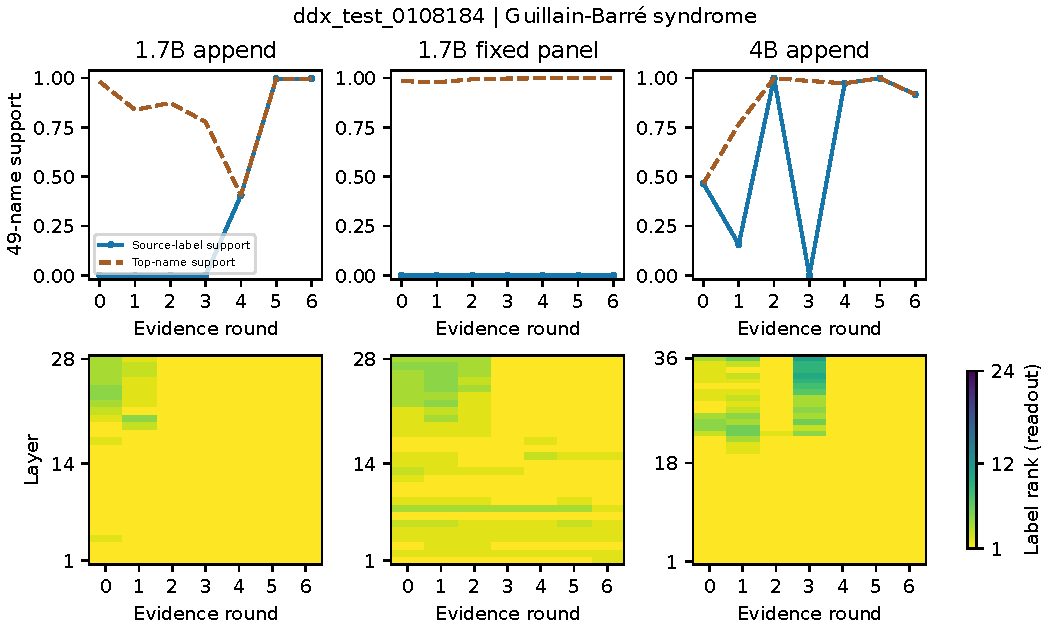
\includegraphics[width=.96\linewidth]{figures/ddx_test_0108184.pdf}\end{center}

{\small\begin{longtable}{>{\raggedright\arraybackslash}p{.07\textwidth}>{\raggedright\arraybackslash}p{.415\textwidth}>{\raggedright\arraybackslash}p{.415\textwidth}}\toprule Round & Newly revealed source evidence & Native top / label support / final-layer probe top \\ \midrule\endhead

0 & Do you currently, or did you ever, have numbness, loss of sensitivity or tingling anywhere on your body? Yes & 1.7B append: Acute COPD exacerbation / infection / 0.0000 / Acute dystonic reactions\newline 1.7B panel: Acute COPD exacerbation / infection / 0.0000 / Myasthenia gravis\newline 4B append: Guillain-Barr\'{e} syndrome / 0.4657 / Possible NSTEMI / STEMI \\ 

1 & Have you traveled out of the country in the last 4 weeks? No & 1.7B append: Acute rhinosinusitis / 0.0000 / Acute dystonic reactions\newline 1.7B panel: Acute COPD exacerbation / infection / 0.0000 / Myasthenia gravis\newline 4B append: Acute rhinosinusitis / 0.1571 / Possible NSTEMI / STEMI \\ 

2 & Do you feel weakness in both arms and/or both legs? Yes & 1.7B append: Bronchiolitis / 0.0000 / Guillain-Barr\'{e} syndrome\newline 1.7B panel: Acute COPD exacerbation / infection / 0.0000 / Myasthenia gravis\newline 4B append: Guillain-Barr\'{e} syndrome / 1.0000 / Guillain-Barr\'{e} syndrome \\ 

3 & Are you experiencing shortness of breath or difficulty breathing in a significant way? Yes & 1.7B append: Acute pulmonary edema / 0.0000 / Guillain-Barr\'{e} syndrome\newline 1.7B panel: Acute pulmonary edema / 0.0000 / Guillain-Barr\'{e} syndrome\newline 4B append: Pulmonary embolism / 0.0000 / Acute pulmonary edema \\ 

4 & Have you recently had numbness, loss of sensation or tingling, in both arms and legs and around your mouth? Yes & 1.7B append: Guillain-Barr\'{e} syndrome / 0.4066 / Guillain-Barr\'{e} syndrome\newline 1.7B panel: Acute pulmonary edema / 0.0000 / Guillain-Barr\'{e} syndrome\newline 4B append: Guillain-Barr\'{e} syndrome / 0.9741 / Guillain-Barr\'{e} syndrome \\ 

5 & Did you previously, or do you currently, have any weakness/paralysis in one or more of your limbs or in your face? Yes & 1.7B append: Guillain-Barr\'{e} syndrome / 0.9965 / Guillain-Barr\'{e} syndrome\newline 1.7B panel: Acute pulmonary edema / 0.0000 / Guillain-Barr\'{e} syndrome\newline 4B append: Guillain-Barr\'{e} syndrome / 0.9998 / Guillain-Barr\'{e} syndrome \\ 

6 & Have you recently had a viral infection? Yes & 1.7B append: Guillain-Barr\'{e} syndrome / 0.9973 / Guillain-Barr\'{e} syndrome\newline 1.7B panel: Acute pulmonary edema / 0.0000 / Guillain-Barr\'{e} syndrome\newline 4B append: Guillain-Barr\'{e} syndrome / 0.9173 / Guillain-Barr\'{e} syndrome \\ 

\bottomrule\end{longtable}}

\clearpage\subsection{ddx\_test\_0110714 -- Pulmonary embolism}
\label{case:ddx_test_0110714}

Source label: Pulmonary embolism. Family: respiratory. Evidence updates: 8. All facts below are source-recorded; their order is acquisition order.

\begin{center}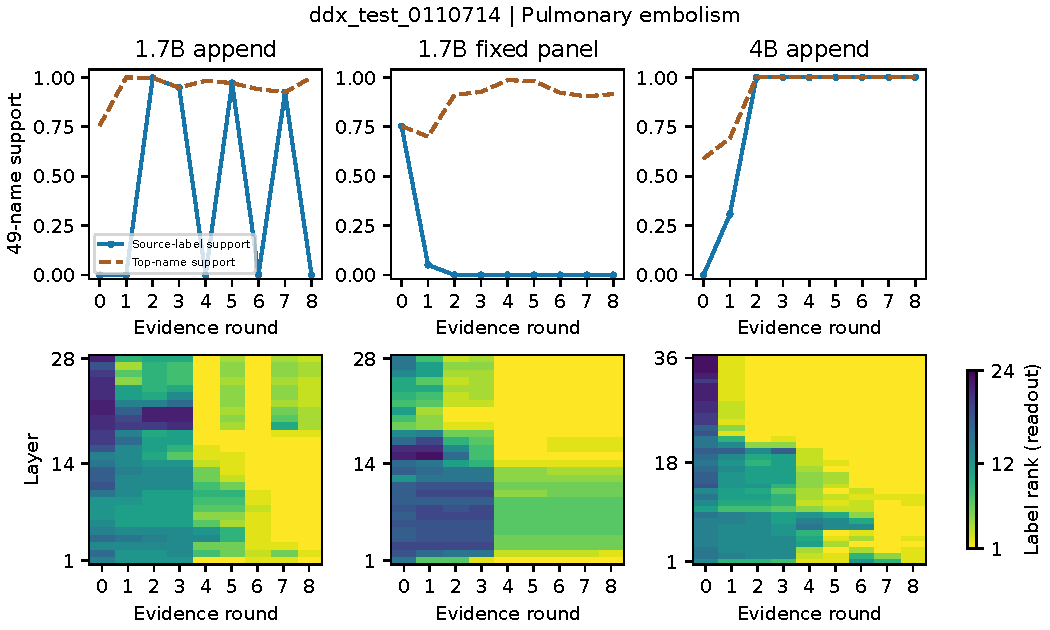
\includegraphics[width=.96\linewidth]{figures/ddx_test_0110714.pdf}\end{center}

{\small\begin{longtable}{>{\raggedright\arraybackslash}p{.07\textwidth}>{\raggedright\arraybackslash}p{.415\textwidth}>{\raggedright\arraybackslash}p{.415\textwidth}}\toprule Round & Newly revealed source evidence & Native top / label support / final-layer probe top \\ \midrule\endhead

0 & Do you have pain that is increased when you breathe in deeply? Yes & 1.7B append: Acute COPD exacerbation / infection / 0.0000 / Bronchitis\newline 1.7B panel: Pulmonary embolism / 0.7534 / SLE\newline 4B append: Acute pulmonary edema / 0.0000 / Bronchitis \\ 

1 & Do you have swelling in one or more areas of your body? Yes; Where is the swelling located? posterior aspect of the ankle(R); posterior aspect of the ankle(L); calf(L) & 1.7B append: Localized edema / 0.0000 / Acute pulmonary edema\newline 1.7B panel: Acute COPD exacerbation / infection / 0.0512 / Myasthenia gravis\newline 4B append: Localized edema / 0.3071 / Acute pulmonary edema \\ 

2 & Have you ever had deep vein thrombosis (DVT)? Yes & 1.7B append: Pulmonary embolism / 0.9975 / Anemia\newline 1.7B panel: Acute COPD exacerbation / infection / 0.0001 / Myasthenia gravis\newline 4B append: Pulmonary embolism / 1.0000 / Pulmonary embolism \\ 

3 & Have you traveled out of the country in the last 4 weeks? North America & 1.7B append: Pulmonary embolism / 0.9483 / Acute pulmonary edema\newline 1.7B panel: Acute COPD exacerbation / infection / 0.0000 / Myasthenia gravis\newline 4B append: Pulmonary embolism / 1.0000 / Pulmonary embolism \\ 

4 & Do you have pain somewhere, related to your reason for consulting? Yes; Characterize your pain: a knife stroke; sharp; Do you feel pain somewhere? side of the chest(R); side of the chest(L); scapula(L); posterior chest wall(R); posterior chest wall(L); How intense is the pain? Recorded scale value 10 on the dataset's 0-10 scale; endpoint meanings are unspecified; Does the pain radiate to another location? side of the chest(R); side of the chest(L); scapula(R); breast(R); posterior chest wall(R); How precisely is the pain located? Recorded scale value 4 on the dataset's 0-10 scale; endpoint meanings are unspecified; How fast did the pain appear? Recorded scale value 10 on the dataset's 0-10 scale; endpoint meanings are unspecified & 1.7B append: Boerhaave / 0.0000 / Pulmonary embolism\newline 1.7B panel: Acute COPD exacerbation / infection / 0.0000 / Pulmonary embolism\newline 4B append: Pulmonary embolism / 1.0000 / Pulmonary embolism \\ 

5 & Did you lose consciousness? Yes & 1.7B append: Pulmonary embolism / 0.9713 / Acute pulmonary edema\newline 1.7B panel: Acute COPD exacerbation / infection / 0.0000 / Pulmonary embolism\newline 4B append: Pulmonary embolism / 1.0000 / Pulmonary embolism \\ 

6 & Have you been coughing up blood? Yes & 1.7B append: Boerhaave / 0.0026 / Pulmonary embolism\newline 1.7B panel: Acute COPD exacerbation / infection / 0.0000 / Pulmonary embolism\newline 4B append: Pulmonary embolism / 1.0000 / Pulmonary embolism \\ 

7 & Have you been unable to move or get up for more than 3 consecutive days within the last 4 weeks? Yes & 1.7B append: Pulmonary embolism / 0.9253 / Acute pulmonary edema\newline 1.7B panel: Acute COPD exacerbation / infection / 0.0000 / Pulmonary embolism\newline 4B append: Pulmonary embolism / 1.0000 / Pulmonary embolism \\ 

8 & Have you had surgery within the last month? Yes & 1.7B append: Localized edema / 0.0001 / Acute pulmonary edema\newline 1.7B panel: Acute COPD exacerbation / infection / 0.0000 / Pulmonary embolism\newline 4B append: Pulmonary embolism / 1.0000 / Pulmonary embolism \\ 

\bottomrule\end{longtable}}

\clearpage\subsection{ddx\_test\_0123136 -- GERD}
\label{case:ddx_test_0123136}

Source label: GERD. Family: digestive. Evidence updates: 8. All facts below are source-recorded; their order is acquisition order.

\begin{center}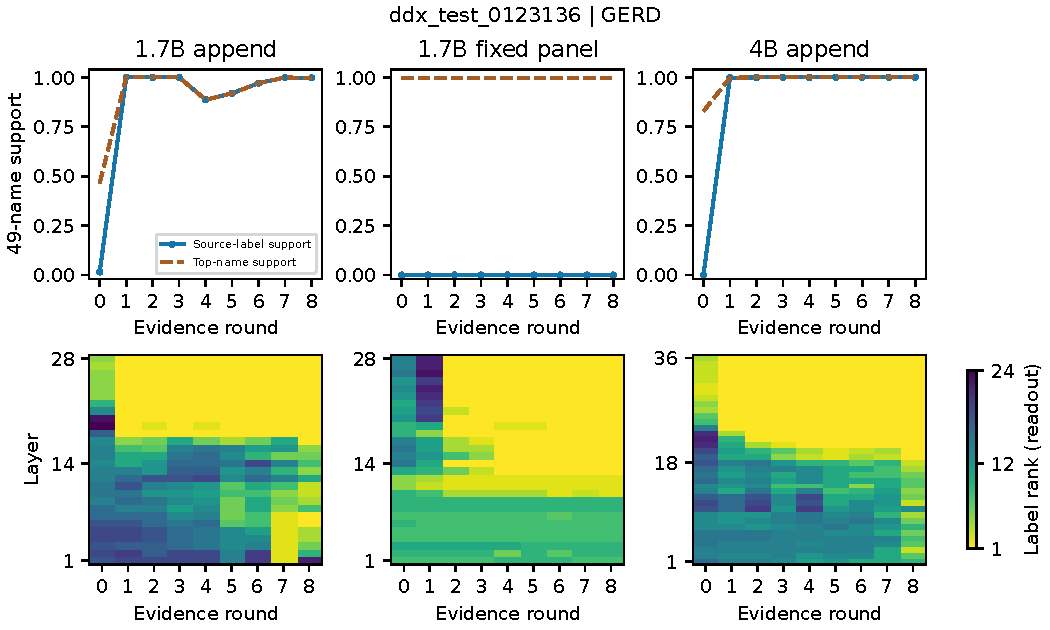
\includegraphics[width=.96\linewidth]{figures/ddx_test_0123136.pdf}\end{center}

{\small\begin{longtable}{>{\raggedright\arraybackslash}p{.07\textwidth}>{\raggedright\arraybackslash}p{.415\textwidth}>{\raggedright\arraybackslash}p{.415\textwidth}}\toprule Round & Newly revealed source evidence & Native top / label support / final-layer probe top \\ \midrule\endhead

0 & Do you have pain somewhere, related to your reason for consulting? Yes; Characterize your pain: sensitive; burning; sickening; scary; Do you feel pain somewhere? upper chest; hypochondrium(L); epigastric; How intense is the pain? Recorded scale value 4 on the dataset's 0-10 scale; endpoint meanings are unspecified; Does the pain radiate to another location? upper chest; How precisely is the pain located? Recorded scale value 2 on the dataset's 0-10 scale; endpoint meanings are unspecified; How fast did the pain appear? Recorded scale value 2 on the dataset's 0-10 scale; endpoint meanings are unspecified & 1.7B append: Acute pulmonary edema / 0.0161 / Stable angina\newline 1.7B panel: Acute COPD exacerbation / infection / 0.0000 / Pericarditis\newline 4B append: Acute pulmonary edema / 0.0000 / Pericarditis \\ 

1 & Do you have a hiatal hernia? Yes & 1.7B append: GERD / 1.0000 / GERD\newline 1.7B panel: Acute COPD exacerbation / infection / 0.0000 / Pericarditis\newline 4B append: GERD / 0.9988 / GERD \\ 

2 & Do you have symptoms that get worse after eating? Yes & 1.7B append: GERD / 1.0000 / GERD\newline 1.7B panel: Acute COPD exacerbation / infection / 0.0000 / GERD\newline 4B append: GERD / 1.0000 / GERD \\ 

3 & Do you think you are pregnant or are you currently pregnant? Yes & 1.7B append: GERD / 1.0000 / GERD\newline 1.7B panel: Acute COPD exacerbation / infection / 0.0000 / GERD\newline 4B append: GERD / 1.0000 / GERD \\ 

4 & Have you recently thrown up blood or something resembling coffee beans? Yes & 1.7B append: GERD / 0.8872 / GERD\newline 1.7B panel: Acute COPD exacerbation / infection / 0.0000 / GERD\newline 4B append: GERD / 1.0000 / GERD \\ 

5 & Do you smoke cigarettes? Yes & 1.7B append: GERD / 0.9196 / GERD\newline 1.7B panel: Acute COPD exacerbation / infection / 0.0000 / GERD\newline 4B append: GERD / 1.0000 / GERD \\ 

6 & Do you have asthma or have you ever had to use a bronchodilator in the past? Yes & 1.7B append: GERD / 0.9707 / GERD\newline 1.7B panel: Acute COPD exacerbation / infection / 0.0000 / GERD\newline 4B append: GERD / 1.0000 / GERD \\ 

7 & Have you traveled out of the country in the last 4 weeks? No & 1.7B append: GERD / 0.9998 / GERD\newline 1.7B panel: Acute COPD exacerbation / infection / 0.0000 / GERD\newline 4B append: GERD / 1.0000 / GERD \\ 

8 & Do you have a burning sensation that starts in your stomach then goes up into your throat, and can be associated with a bitter taste in your mouth? Yes & 1.7B append: GERD / 0.9977 / GERD\newline 1.7B panel: Acute COPD exacerbation / infection / 0.0000 / GERD\newline 4B append: GERD / 1.0000 / GERD \\ 

\bottomrule\end{longtable}}

\clearpage\subsection{ddx\_test\_0134351 -- Viral pharyngitis}
\label{case:ddx_test_0134351}

Source label: Viral pharyngitis. Family: ent. Evidence updates: 5. All facts below are source-recorded; their order is acquisition order.

\begin{center}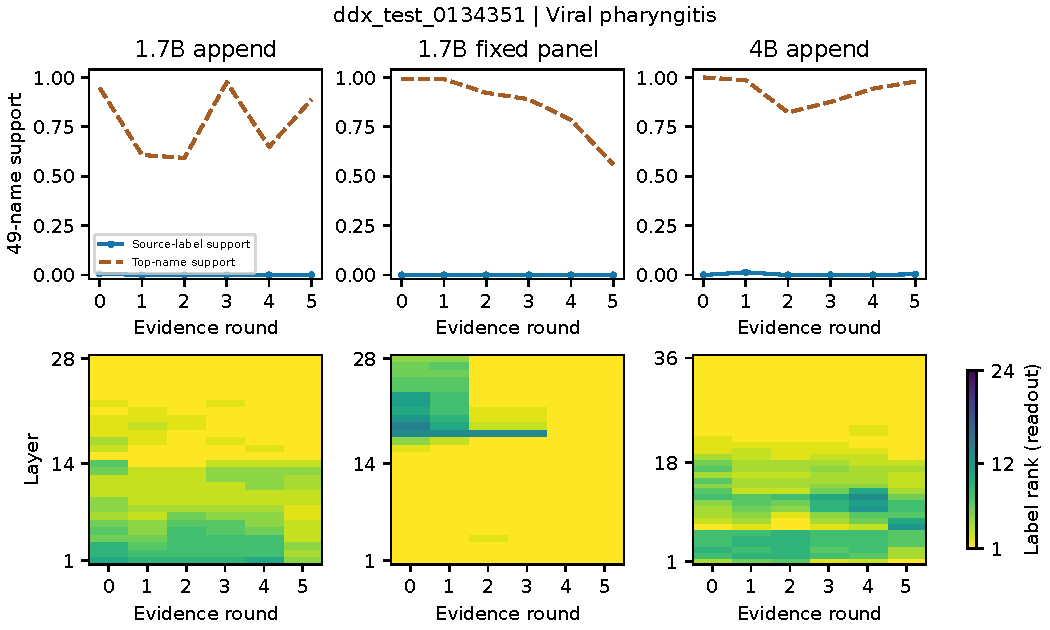
\includegraphics[width=.96\linewidth]{figures/ddx_test_0134351.pdf}\end{center}

{\small\begin{longtable}{>{\raggedright\arraybackslash}p{.07\textwidth}>{\raggedright\arraybackslash}p{.415\textwidth}>{\raggedright\arraybackslash}p{.415\textwidth}}\toprule Round & Newly revealed source evidence & Native top / label support / final-layer probe top \\ \midrule\endhead

0 & Do you have pain somewhere, related to your reason for consulting? Yes; Characterize your pain: sensitive; burning; Do you feel pain somewhere? tonsil(R); tonsil(L); palace; pharynx; under the jaw; How intense is the pain? Recorded scale value 9 on the dataset's 0-10 scale; endpoint meanings are unspecified; Does the pain radiate to another location? nowhere; How precisely is the pain located? Recorded scale value 7 on the dataset's 0-10 scale; endpoint meanings are unspecified; How fast did the pain appear? Recorded scale value 3 on the dataset's 0-10 scale; endpoint meanings are unspecified & 1.7B append: Acute rhinosinusitis / 0.0075 / Viral pharyngitis\newline 1.7B panel: Acute COPD exacerbation / infection / 0.0000 / Acute otitis media\newline 4B append: Acute rhinosinusitis / 0.0001 / Viral pharyngitis \\ 

1 & Do you smoke cigarettes? Yes & 1.7B append: Acute laryngitis / 0.0000 / Viral pharyngitis\newline 1.7B panel: Acute COPD exacerbation / infection / 0.0000 / Acute otitis media\newline 4B append: Acute rhinosinusitis / 0.0141 / Viral pharyngitis \\ 

2 & Have you been coughing up blood? Yes & 1.7B append: Acute rhinosinusitis / 0.0001 / Viral pharyngitis\newline 1.7B panel: Acute COPD exacerbation / infection / 0.0000 / Viral pharyngitis\newline 4B append: Acute rhinosinusitis / 0.0000 / Viral pharyngitis \\ 

3 & Have you traveled out of the country in the last 4 weeks? No & 1.7B append: Acute rhinosinusitis / 0.0025 / Viral pharyngitis\newline 1.7B panel: Acute COPD exacerbation / infection / 0.0000 / Viral pharyngitis\newline 4B append: Acute rhinosinusitis / 0.0003 / Viral pharyngitis \\ 

4 & Are you immunosuppressed? Yes & 1.7B append: GERD / 0.0002 / Viral pharyngitis\newline 1.7B panel: Acute COPD exacerbation / infection / 0.0000 / Viral pharyngitis\newline 4B append: Pneumonia / 0.0000 / Viral pharyngitis \\ 

5 & Have you been in contact with a person with similar symptoms in the past 2 weeks? Yes & 1.7B append: Acute rhinosinusitis / 0.0002 / Viral pharyngitis\newline 1.7B panel: Acute COPD exacerbation / infection / 0.0000 / Viral pharyngitis\newline 4B append: Pneumonia / 0.0042 / Viral pharyngitis \\ 

\bottomrule\end{longtable}}
